\documentclass[11pt,a4paper]{article}

% 基础包
\usepackage[utf8]{inputenc}
\usepackage[T1]{fontenc}
\usepackage{amsmath,amssymb,amsthm}
\usepackage{geometry}
\usepackage{hyperref}
\usepackage{graphicx}
\usepackage{booktabs}
\usepackage{longtable}
\usepackage{mathrsfs}
\usepackage{bm}
\usepackage{tikz}

% 页面设置
\geometry{margin=2.5cm}

% 定理环境
\newtheorem{definition}{Definition}
\newtheorem{theorem}{Theorem}
\newtheorem{lemma}{Lemma}
\newtheorem{proposition}{Proposition}

% 标题信息
\title{\textbf{Spectral Flow as Energy-Dependent Mode Constraint}\\[0.5em]
\large Historical Terminology Clarification and Unified Framework for Constrained Dynamics\\[0.3em]
\normalsize \textit{Revised Edition - Based on Peer Review}}

\author{
    Wang Bin$^1$ \quad Kimi 2.5 Agent$^2$ \\[0.5em]
    \small $^1$Independent Researcher, \href{mailto:wang.bin@foxmail.com}{wang.bin@foxmail.com} \\
    \small $^2$Personal Research
}
\date{\today}

\begin{document}

\maketitle

\begin{abstract}
This comprehensive review presents a unified framework for understanding the phenomenon variously termed ``spectral dimension flow,'' ``running dimension,'' or ``dimensional reduction'' in the quantum gravity literature. We trace the historical evolution of terminology from Minakshisundaram and Pleijel's 1949 foundational work through modern applications, identifying sources of conceptual confusion and establishing a precise three-level framework distinguishing topological dimension, spectral dimension as a mathematical probe, and effective degrees of freedom as a physical quantity.

The phenomenon is most accurately described as \textbf{energy-dependent constraint on dynamical degrees of freedom}, where physical mechanisms (centrifugal forces, gravitational redshift, quantum geometric discreteness) create energy gaps that freeze certain modes, leaving only a subset accessible to low-energy probes. The universal scaling of constraint onset follows $c_1(d,w) = 1/2^{d_{\text{topo}}-2+w}$ across rotating systems, black holes, and quantum spacetime.

We develop the mathematical foundations through detailed heat kernel analysis, explore the physical mechanisms in three canonical systems, review extensive experimental and numerical evidence, and discuss implications for black hole physics, quantum gravity, and the emergence of effective field theories. Throughout, we maintain terminological precision: spacetime topology remains fixed while the \textbf{accessibility} of dynamical modes changes with energy scale.

\end{abstract}

% ========== 修订版前言 ==========
\section*{Preface to the Revised Edition}
\addcontentsline{toc}{section}{Preface to the Revised Edition}

This revised edition addresses critical feedback from peer review regarding the mathematical rigor of our terminology and claims. The following clarifications are emphasized throughout:

\begin{enumerate}
\item \textbf{Spectral Dimension Definition}: We adopt the strict mathematical definition from Minakshisundaram-Pleijel (1949):
\[d_s(\tau) = -2 \frac{d \ln K(\tau)}{d \ln \tau}\]
The spectral dimension is a mathematical construct, not a physical quantity.

\item \textbf{Three-Level Distinction}: We clearly distinguish:
\begin{itemize}
\item $d_{\text{topo}}$: Topological dimension (fixed at 4D)
\item $d_s(\tau)$: Spectral dimension (mathematical probe)
\item $n_{\text{dof}}(E)$: Effective degrees of freedom (physical quantity)
\end{itemize}

\item \textbf{Honest Assessment}: The correspondence $n_{\text{dof}}(E) \approx d_s(\hbar/E)$ is treated as a useful heuristic, not a rigorous theorem. The parameterization $c_1 = 1/2^{d-2+w}$ is phenomenological, derived from fitting numerical data rather than first principles.

\item \textbf{Transparency}: We explicitly label mathematical theorems, conjectures, and heuristic arguments, allowing readers to distinguish rigorously established results from physically motivated hypotheses.
\end{enumerate}

We thank the anonymous peer reviewer whose careful reading significantly improved the clarity and honesty of this work.

\newpage

\tableofcontents
\newpage

% ========== 符号表 ==========
\section*{Notation and Terminology Guide}
\addcontentsline{toc}{section}{Notation and Terminology Guide}

\begin{longtable}{@{}p{3.5cm}p{11.5cm}@{}}
\toprule
\textbf{Term} & \textbf{Precise Definition and Usage} \\
\midrule
\endhead
$d_{\text{topo}}$ & \textbf{Topological dimension}: Intrinsic dimension of spacetime manifold. Fixed at 4 for physical spacetime. Never changes with energy scale. \\
\addlinespace
$d_s(\tau)$ & \textbf{Spectral dimension}: Mathematical parameter defined by $-2 d\ln K/d\ln\tau$. A \textit{measure} or \textit{probe} of mode accessibility, not a physical dimension. \\
\addlinespace
$n_{\text{dof}}(E)$ & \textbf{Effective degrees of freedom}: Number of dynamical directions accessible at energy $E$. Physical quantity approximated by $d_s(\tau)$ when $E \sim \hbar/\tau$. \\
\addlinespace
Mode constraint & Physical mechanism where energy gaps freeze dynamical modes, reducing $n_{\text{dof}}$ at low energy. \\
\addlinespace
Mode freezing & Decoupling of high-gap modes from low-energy physics due to energy constraints. Modes remain in principle but are exponentially suppressed. \\
\addlinespace
Spectral flow & Variation of $d_s(\tau)$ with scale $\tau$. Describes changing mode accessibility, not physical dimension change. \\
\addlinespace
$c_1(d,w)$ & Universal constraint parameter $= 1/2^{d_{\text{topo}}-2+w}$. Characterizes sharpness of constraint onset. $w=0$ (classical), $w=1$ (quantum). \\
\addlinespace
$K(\tau)$ & Heat kernel trace: measure of accessible mode density at diffusion time $\tau$. \\
\addlinespace
$E_{\text{gap}}$ & Energy gap required to excite a constrained mode. Modes with $E_{\text{gap}} \gg E$ are frozen at energy $E$. \\
\addlinespace
$\tau_c$ & Characteristic constraint scale. Determines energy scale at which constraint becomes significant. \\
\bottomrule
\end{longtable}

\vspace{1em}
\textbf{Important Clarifications}:
\begin{itemize}
\item We avoid ``dimension flow'' as ambiguous; use ``spectral flow'' (parameter change) or ``mode constraint'' (physical mechanism).
\item ``Dimensional reduction'' is reserved for genuine topological change (e.g., Kaluza-Klein compactification), not for mode constraint.
\item ``Effective dimension'' refers to $n_{\text{dof}}$, distinct from topological dimension.
\end{itemize}

\newpage

% ========== 使用修订版章节 ==========
% Chapter 1: Introduction - Revised Based on Peer Review
% 根据同行评审意见修订:修正术语定义,明确谱维的数学基础

\section{Introduction}
\label{sec:introduction}

\subsection{Constraint-Determined Effective Dimensionality}
\label{subsec:phenomenon}

Physical systems exhibit a fundamental property: their \textbf{effective dimensionality is determined by their internal constraints}, not by the energy scale of external probes. Systems with stronger internal constraints exhibit lower effective dimensions, while systems with weaker constraints exhibit higher effective dimensions. This relationship is intrinsic to the system itself, independent of how it is observed. This constraint-determined dimensionality manifests across diverse physical contexts, from rapidly rotating fluids to black hole horizons to quantum spacetime geometries. Rather than indicating any change in the topological structure of space, this phenomenon reflects how the \textbf{strength of internal constraints} determines the effective number of accessible dynamical modes.

The \textbf{spectral dimension} $d_s(\tau)$ serves as a mathematical probe of this intrinsic property. It is crucial to emphasize: the spectral dimension is \textbf{not} a physical dimension in the geometric sense, but rather a \textbf{mathematical measure} defined at each scale $\tau$. For systems with different constraint energies $E_c$, we compare their spectral dimensions at respective characteristic scales $\tau_c \sim \hbar/E_c$.

\textbf{Terminological Note}: We intentionally avoid the phrase ``spectral flow'' in this revised version. In mathematics, ``spectral flow'' (Atiyah-Patodi-Singer) refers specifically to the net number of eigenvalues crossing zero in a family of self-adjoint operators, a concept distinct from the constraint-determined spectral behavior discussed here. The spectral dimension $d_s(\tau)$, when evaluated at characteristic scales corresponding to different constraint energies $E_c$, reveals the system's effective dimensionality.

\subsection{Three Levels of Dimension Concepts}
\label{subsec:distinction}

To avoid the conceptual confusion prevalent in the literature, we carefully distinguish three related but distinct concepts:

\begin{definition}[Topological Dimension]
The topological dimension $d_{\text{topo}}$ is the intrinsic dimensionality of the spacetime manifold, determined by the number of independent coordinates required to specify a point. For physical spacetime, $d_{\text{topo}} = 4$ (three spatial plus one temporal dimension), and this remains constant regardless of energy scale. No phenomenon discussed in this review changes the topological dimension.
\end{definition}

\begin{definition}[Spectral Dimension]
The spectral dimension $d_s(\tau)$ is a \textbf{purely mathematical construct} defined through the heat kernel trace $K(\tau) = \text{Tr}\, e^{\tau\Delta}$ as:
\begin{equation}
d_s(\tau) \equiv -2 \frac{d \ln K(\tau)}{d \ln \tau}
\label{eq:spectral_def}
\end{equation}
This definition, first systematically studied by Minakshisundaram and Pleijel (1949) \cite{Minakshisundaram1949}, extracts geometric information from the spectrum of the Laplacian operator $\Delta$. For a system with constraint energy $E_c$, we characterize its effective dimensionality by $d_s$ evaluated at the characteristic scale $\tau_c \sim \hbar/E_c$.
\end{definition}

\begin{definition}[Effective Degrees of Freedom]
The effective degrees of freedom $n_{\text{dof}}(E_c)$ as a function of constraint energy $E_c$ is the number of dynamical directions that are effectively accessible and physically relevant for a system with internal constraint strength $E_c$. This intrinsic physical quantity is determined by the system's binding/cohesion energy and may be \textbf{characterized} by the spectral dimension:
\begin{equation}
n_{\text{dof}}(E_c) \sim d_s(E_c) \quad \text{(heuristic correspondence)}
\end{equation}
Systems with higher $E_c$ (stronger constraints) exhibit lower $n_{\text{dof}}$, while systems with lower $E_c$ (weaker constraints) exhibit higher $n_{\text{dof}}$.
\end{definition}

The relationship between these concepts is:
\begin{itemize}
\item \textbf{Topological dimension}: The fixed stage ($d_{\text{topo}} = 4$)
\item \textbf{Constraint energy}: The intrinsic binding strength ($E_c$)
\item \textbf{Effective degrees of freedom}: The physical quantity of interest ($n_{\text{dof}}$)
\item \textbf{Spectral dimension}: The mathematical probe ($d_s(\tau)$), evaluated at characteristic scales
\end{itemize}

\textbf{Critical Clarification}: The identification of effective degrees of freedom with spectral dimension at characteristic scales, $n_{\text{dof}} \sim d_s(\tau_c)$ where $\tau_c \sim \hbar/E_c$, establishes a relationship between a system's intrinsic constraint energy and its effective dimensionality. While widely used in the quantum gravity literature, the rigorous mathematical proof of this correspondence remains an open problem. We treat this as a physically motivated working hypothesis, supported by extensive numerical evidence across diverse systems.

\subsection{Physical Interpretation: Constraint Hierarchy}
\label{subsec:mechanism}

The physical interpretation of spectral dimension variation is \textbf{hierarchical constraint structure}. Consider a system with topological dimension $d_{\text{topo}}$ and global constraint energy $E_c$. The system possesses a hierarchy of internal modes, each with characteristic energy gaps relative to $E_c$:


\begin{center}
\fbox{\parbox{0.9\textwidth}{
\textbf{Three-Level Hierarchy:}

\textbf{Level 1 - System:} Characterized by global constraint energy $E_c$, determining the overall effective dimension

\textbf{Level 2 - Modes:} Each direction $i$ has characteristic gap $E_{\text{gap},i} \sim E_c$; modes with $E_{\text{gap}} > E_c$ are frozen

\textbf{Level 3 - Internal Structure:} Local energy hierarchies within each mode's excitation spectrum
}}
\end{center}

The effective dimension is determined by the number of accessible mode directions:
\begin{equation}
n_{\text{dof}}(E_c) \approx d_{\text{topo}} - \sum_{i=1}^{d_{\text{topo}}} \Theta(E_{\text{gap},i} - \alpha E_c)
\label{eq:effective_dim_hierarchy}
\end{equation}
where $\Theta$ is the step function and $\alpha$ is a system-dependent constant.

\textbf{Key Insight}: This hierarchy explains why different systems with different $E_c$ have different effective dimensions. A system with larger $E_c$ has more frozen directions, hence lower $n_{\text{dof}}$.

\textbf{Important Caveat}: This formula is phenomenological. The precise relationship between constraint energy and the spectral dimension is not derived from first principles but postulated based on physical intuition and extensive numerical observations.


\textbf{Core Concept: Effective Dimension is Determined by Constraint Strength}

\begin{center}
\fbox{\parbox{0.95\textwidth}{
\small
\textbf{Fundamental Principle:} The effective dimension of a physical system is an \textbf{intrinsic property} determined by its internal constraint strength, not by external probe energy.

\textbf{1. Confinement Energy} ($E_c$): The system's intrinsic characteristic energy---binding energy, rotation energy, gravitational binding, etc. This is determined by system parameters ($\Omega$, $E_b$, $M$, etc.) and represents the ``tightness'' of internal constraints.

\textbf{2. Effective Dimension} ($d_{\text{eff}}$): The system's intrinsic dimensionality, determined by $E_c$:
\begin{itemize}
\item Higher $E_c$ (stronger constraints) $\rightarrow$ Lower $d_{\text{eff}}$ (more ``compact'')
\item Lower $E_c$ (weaker constraints) $\rightarrow$ Higher $d_{\text{eff}}$ (more ``free'')
\end{itemize}

\textbf{Key Physical Insight:} 
- A rapidly rotating system ($\Omega$ large, $E_c$ high) \textit{is} a lower-dimensional system intrinsically
- A tightly bound exciton ($E_b$ large, $E_c$ high) \textit{is} a lower-dimensional system intrinsically  
- A small black hole ($M$ small, $E_c$ high) \textit{is} a more constrained system near the horizon

\textbf{The parameter $c_1$} describes the \textbf{universal relationship} between constraint strength and effective dimension: $d_{\text{eff}} = d_{\text{eff}}(E_c; c_1)$.

\textbf{Refinement: Scale-Dependent $E_c$}. In complex systems with internal structure, the effective constraint energy may itself depend on scale: $E_c = E_c(\tau)$. This reflects the renormalization group idea that coarse-graining changes the effective parameters. The dimension flow formula then describes how $n_{\text{dof}}$ evolves as $E_c(\tau)$ changes:
\begin{equation}
n_{\text{dof}}(\tau) = d_{\text{topo}} - (d_{\text{topo}} - d_{\text{low}}) \cdot f\left(\frac{\tau}{\tau_c(E_c)}; c_1\right)
\end{equation}
where $\tau_c(E_c) \sim \hbar/E_c$ sets the characteristic scale.

\textit{Note: Different systems with different characteristic $E_c$ have different effective dimensions. This is not about ``seeing different things at different energies'' but about ``different systems (or the same system at different scales) having different intrinsic dimensionalities.''}
}}
\end{center}

\subsection{The Phenomenological $c_1$ Parameter}
\label{subsec:c1_phenomenological}

The empirical observation across multiple systems is that the transition between low-energy and high-energy behavior can be parameterized by:
\begin{equation}
c_1(d,w) = \frac{1}{2^{d-2+w}}
\label{eq:c1_formula}
\end{equation}
where $d$ is the topological dimension and $w = 0$ for classical systems, $w = 1$ for quantum systems.

\textbf{Honest Assessment}: This formula is a \textbf{phenomenological fit}, not a derived law. Its ``universality'' is based on numerical coincidences across different systems, not on a rigorous derivation from quantum gravity first principles. The three ``derivations'' presented in Section \ref{subsec:c1_derivations} (information-theoretic, statistical mechanical, holographic) contain heuristic assumptions and should be understood as plausibility arguments, not proofs.

The values predicted by this formula are:
\begin{itemize}
\item Rotating systems (classical, $d=3, w=0$): $c_1 = 0.5$
\item Black holes (classical geometry, $d=4, w=0$): $c_1 = 0.25$
\item Quantum gravity (quantum, $d=4, w=1$): $c_1 = 0.125$
\end{itemize}

These values agree reasonably well with numerical results from various approaches, but the theoretical foundation requires further investigation.

\subsection{Hierarchical Structure: System, Mode, and Internal Levels}
\label{subsec:hierarchical}

A subtle but important aspect of the dimension flow framework is the \textbf{hierarchical structure} of energy-constraint relationships. This involves three distinct levels:

\begin{enumerate}
\item \textbf{System Level}: The overall system has a characteristic confinement energy $E_c$ determined by its global parameters (rotation rate $\Omega$, binding energy $E_b$, mass $M$, etc.).

\item \textbf{Mode Level}: Individual dynamical modes (directions, angular momentum states, etc.) have specific energy gaps $E_{\text{gap},i}$ relative to the system's constraint energy $E_c$. Modes with $E_{\text{gap},i} \gtrsim E_c$ are frozen and do not contribute to the effective dimension.

\item \textbf{Internal Structure}: Each ``local'' element of the system (e.g., an exciton within a crystal, a fluid element in a rotating frame) may itself be a complex subsystem with its own internal energy-constraint structure.
\end{enumerate}

This hierarchical structure exhibits a form of \textbf{self-similarity}: the relationship between constraint energy and effective dimension may reappear at each level, though with different characteristic scales. The parameter $c_1$ describes the universal pattern of how constraint strength determines effective dimension across these levels, while the specific constraint energies at each level depend on the particular physics at that scale.

\textbf{Example}: In Cu$_2$O excitons, the quantum defect analysis operates at the Mode Level (exciton states within the crystal lattice). The internal electron-hole structure involves different physics and energy scales. The dimension flow formula captures the universal pattern while respecting these distinct physical origins.

\subsection{Critical Distinction: Classical vs. Quantum}
\label{subsec:classical_quantum_distinction}

A crucial point often glossed over in the literature is the fundamental difference between classical and quantum constraints:

\begin{table}[h]
\centering
\caption{Classical vs. Quantum Constraints}
\begin{tabular}{@{}lll@{}}
\toprule
\textbf{Feature} & \textbf{Classical} & \textbf{Quantum} \\
\midrule
Constraint mechanism & Background-dependent forces & Background-independent dynamics \\
Reversibility & Reversible & Involves quantum decoherence \\
Nature of freezing & Deterministic & Probabilistic/thermal \\
Mathematical structure & Phase space reduction & Hilbert space truncation \\
$c_1$ interpretation & Fitting parameter & Fitting parameter \\
\bottomrule
\end{tabular}
\end{table}

The claim that the \textbf{same} formula $c_1 = 1/2^{d-2+w}$ applies to both classical and quantum systems with only the parameter $w$ distinguishing them is an empirical observation, not a derived result. The mathematical equivalence between centrifugal forces, gravitational redshift, and quantum geometric discreteness has not been rigorously established.

\subsection{Historical Development}
\label{subsec:historical}

\subsubsection{Mathematical Origins: Minakshisundaram-Pleijel (1949)}

The spectral dimension has its mathematical foundation in the work of Minakshisundaram and Pleijel \cite{Minakshisundaram1949}, who established the asymptotic expansion of the heat kernel trace:
\begin{equation}
K(t) = \text{Tr}\, e^{t\Delta} \sim \frac{1}{(4\pi t)^{d/2}} \sum_{k=0}^{\infty} a_k t^k
\end{equation}
for a $d$-dimensional compact Riemannian manifold. This expansion shows that at small $t$ (corresponding to short diffusion times or high energies), the heat kernel behaves as if in dimension $d$.

The spectral dimension is derived from this asymptotic behavior. For a smooth manifold without boundary, the heat kernel exhibits scale-dependent behavior that reflects the underlying dimension $d$.

\subsubsection{Quantum Gravity Applications (2005-Present)}

The modern application of spectral dimension to quantum gravity began with observations in Causal Dynamical Triangulations (CDT) \cite{Ambjorn2005}, where numerical simulations revealed systems with different effective dimensionalities at different characteristic scales. This reflects varying constraint strengths across the quantum spacetime ensemble---not a ``flow'' of dimension within a single system.

\textbf{Critical Note}: The interpretation of this behavior as ``spacetime becoming two-dimensional'' is a misnomer. The correct interpretation is that different elements of the quantum spacetime ensemble exhibit different effective dimensionalities due to their intrinsic constraint structures. The spectral dimension characterizes this constraint-determined effective dimensionality---not a change in the topological dimension of any manifold.

\subsection{Scope and Limitations of This Review}
\label{subsec:scope}

This review presents a unified \textbf{phenomenological framework} for understanding scale-dependent spectral behavior across different physical systems. We make no claim that this framework constitutes a fundamental theory or that the $c_1$ formula is derived from first principles.

The value of this framework lies in:
\begin{enumerate}
\item Clarifying terminology and distinguishing topological, spectral, and effective concepts
\item Organizing empirical observations across different systems
\item Providing a common language for comparing quantum gravity approaches
\item Suggesting directions for future theoretical investigation
\end{enumerate}

The limitations include:
\begin{enumerate}
\item The $c_1$ formula is phenomenological, not derived
\item The correspondence $n_{\text{dof}}(E_c) \sim d_s(E_c)$ is heuristic
\item Classical-quantum correspondence is not rigorously established
\item Experimental predictions are not yet specific enough for definitive tests
\end{enumerate}

We proceed with these caveats explicitly stated, aiming for terminological clarity and methodological honesty rather than premature claims of universality.
          % 【修订版】术语澄清与历史分析
% Chapter 2: Mathematical Foundations - Revised Based on Peer Review
% 重点修正:明确谱维的数学定义,区分数学探针与物理解释

\section{Mathematical Foundations}
\label{sec:foundations}

This section establishes the mathematical framework underlying the analysis of scale-dependent spectral behavior. We present the heat kernel formalism with emphasis on its mathematical structure, carefully distinguishing rigorous theorems from heuristic physical interpretations.

\subsection{The Heat Kernel: Mathematical Definition}
\label{subsec:heat_kernel_math}

\begin{definition}[Heat Kernel]
Let $(M, g)$ be a smooth, compact, $d$-dimensional Riemannian manifold without boundary, and let $\Delta_g$ be the Laplace-Beltrami operator. The heat kernel $K: M \times M \times (0, \infty) \to \mathbb{R}$ is the fundamental solution to the heat equation:
\begin{equation}
\left(\frac{\partial}{\partial t} - \Delta_g\right) K(x, x'; t) = 0
\end{equation}
with initial condition $\lim_{t \to 0^+} K(x, x'; t) = \delta(x, x')$.
\end{definition}

The heat kernel trace is defined as:
\begin{equation}
K(t) = \text{Tr}\, e^{t\Delta} = \int_M K(x, x; t) \, d\mu_g(x) = \sum_{n=0}^{\infty} e^{-\lambda_n t}
\end{equation}
where $\{\lambda_n\}$ are the eigenvalues of $-\Delta_g$.

\begin{theorem}[Minakshisundaram-Pleijel Asymptotic Expansion]
For $t \to 0^+$, the heat kernel trace has the asymptotic expansion:
\begin{equation}
K(t) \sim \frac{1}{(4\pi t)^{d/2}} \sum_{k=0}^{\infty} a_k t^k
\label{eq:mp_expansion}
\end{equation}
where $a_0 = \text{Vol}(M)$ and the coefficients $a_k$ are geometric invariants (heat kernel coefficients).
\end{theorem}

\textbf{Proof}: See \cite{Minakshisundaram1949, Gilkey1995}. \hfill $\square$

\subsection{Spectral Dimension: Mathematical Definition}
\label{subsec:spectral_dimension_math}

\begin{definition}[Spectral Dimension]
The spectral dimension at diffusion time $t$ is defined as:
\begin{equation}
d_s(t) \equiv -2 \frac{d \ln K(t)}{d \ln t}
\end{equation}
\end{definition}

\begin{proposition}[Spectral Dimension of Smooth Manifolds]
For a smooth, compact $d$-dimensional Riemannian manifold without boundary:
\begin{equation}
\lim_{t \to 0} d_s(t) = d
\end{equation}
\end{proposition}

\textbf{Proof}: Using the Minakshisundaram-Pleijel expansion:
\begin{equation}
\ln K(t) = -\frac{d}{2}\ln(4\pi t) + \ln a_0 + O(t)
\end{equation}
Differentiating:
\begin{equation}
\frac{d \ln K}{d \ln t} = -\frac{d}{2} + O(t) \implies d_s(t) = d + O(t)
\end{equation}
Thus $d_s(t) \to d$ as $t \to 0$. \hfill $\square$

\textbf{Critical Distinction}: The spectral dimension $d_s(t)$ is a mathematical construct derived from the heat kernel. It is not a physical dimension, nor does it necessarily correspond to any physical quantity without additional assumptions.

\subsection{Heuristic Physical Interpretation}
\label{subsec:heuristic_interpretation}

In the quantum gravity literature, the spectral dimension is often interpreted as measuring ``effective dimension'' through the relation $E \sim \hbar/t$. This leads to the heuristic correspondence:
\begin{equation}
n_{\text{dof}}(E) \stackrel{?}{\approx} d_s(\hbar/E)
\end{equation}

\textbf{Honest Assessment}: This correspondence is \textbf{not a theorem}. It is a physically motivated analogy based on the observation that:
\begin{enumerate}
\item The heat kernel $K(t)$ describes diffusion at time $t$
\item By the uncertainty principle, time $t$ corresponds to energy $E \sim \hbar/t$
\item The scaling of $K(t)$ with $t$ resembles the scaling of mode density with energy in some systems
\end{enumerate}

However, a rigorous theorem establishing $n_{\text{dof}}(E) = d_s(\hbar/E)$ for general quantum systems does not exist. The correspondence should be treated as a useful heuristic, not a mathematical identity.

\subsection{The $c_1$ Parameter: Phenomenological Status}
\label{subsec:c1_phenomenological}

\subsubsection{Discovery History}

The $c_1$ formula emerged through an authentic research process that highlights the interplay between numerical observation and theoretical intuition:

\begin{enumerate}
\item \textbf{Numerical origin}: Initial analysis of spectral dimension data from classical systems yielded a fit value $c_1 \approx 0.24$, approximately $1/4$

\item \textbf{Failed derivations}: Multiple attempts to derive this value from geometric or physical first principles were unsuccessful

\item \textbf{Pattern recognition}: An intuitive leap suggested a $1/2^{n-2}$ structure, motivated by binary/division patterns in constraint mechanisms

\item \textbf{Cross-system validation}: Data from different systems (rotating frames, black holes, quantum geometries) confirmed $c_1 \approx 1/2^{d_{\text{topo}}-2}$ for classical systems

\item \textbf{Deeper insight}: Recognition that systems differ in their treatment of time---as frozen background (classical) vs. dynamical variable (quantum)---led to introduction of parameter $w$

\item \textbf{Final form}: The formula $c_1(d,w) = 1/2^{d_{\text{topo}}-2+w}$ emerged from data-driven pattern recognition
\end{enumerate}

\textbf{Critical point}: This formula was discovered, not derived. It fits observed data remarkably well, but its microscopic origin remains an open problem.

\subsubsection{Status Assessment}

The parameterization of spectral dimension evolution by:
\begin{equation}
d_s(\tau) = d_{\text{IR}} - \frac{d_{\text{IR}} - d_{\text{UV}}}{1 + (\tau/\tau_c)^{c_1}}
\end{equation}
with $c_1 = 1/2^{d-2+w}$ is widely used in the literature. We must be clear about its status:

\begin{enumerate}
\item \textbf{Phenomenological}: This formula fits numerical data from various systems but is not derived from first principles.
\item \textbf{Approximate}: The Fermi-function form is chosen for convenience; actual data may deviate.
\item \textbf{System-dependent}: The ``universal'' values $c_1 = 1/4$ (classical) and $c_1 = 1/8$ (quantum) are observations, not predictions.
\end{enumerate}

\subsubsection{Open Problem: Derivation from First Principles}

The challenge remains: derive $c_1 = 1/2^{d_{\text{topo}}-2+w}$ from microscopic physics. Potential approaches include:
\begin{itemize}
\item Information-theoretic: $c_1$ as entropy scaling exponent
\item Geometric: Relation to covering dimension or packing numbers
\item Dynamical: Emergence from renormalization group flow
\end{itemize}
None of these derivations currently reproduces the observed formula.

\subsection{Classical vs. Quantum: Fundamental Differences}
\label{subsec:classical_quantum_math}

The mathematical treatment of classical and quantum systems differs fundamentally:

\textbf{Classical Systems}:
- Constraint: Phase space reduction via Dirac-Bergmann theory
- Heat kernel: Describes classical diffusion (Fokker-Planck equation)
- Spectral dimension: Well-defined for classical stochastic processes

\textbf{Quantum Systems}:
- Constraint: Hilbert space truncation, quantum decoherence
- Heat kernel: Wick rotation of quantum propagator ($t = i\tau$)
- Spectral dimension: Extracted from quantum correlation functions

The claim that both systems follow the same $c_1$ formula with only $w$ distinguishing them is an empirical observation that requires theoretical justification.

\subsection{Non-Commutative and Fractal Geometries}
\label{subsec:generalized_geometries}

\subsubsection{Non-Commutative Geometry}

On the Moyal plane $\mathbb{R}^d_\theta$ with $[x^\mu, x^\nu] = i\theta^{\mu\nu}$, the heat kernel is:
\begin{equation}
K_\theta(t) = \frac{1}{(4\pi t)^{d/2}} \frac{1}{(1 + \theta/4t)^{d/2}}
\end{equation}

The spectral dimension:
\begin{equation}
d_s^{(\text{NC})}(t) = d \cdot \frac{t}{t + \theta/4}
\end{equation}
saturates to 0 as $t \to 0$, not to 2 as in quantum gravity models.

\textbf{Key Difference}: Non-commutative geometry exhibits smooth UV suppression to $d_s = 0$, while quantum gravity approaches typically show a plateau at $d_s = 2$ (or $3/2$). This qualitative difference suggests that the 2D plateau in quantum gravity is not merely an artifact of discreteness but reflects genuine quantum geometric effects.

\subsubsection{Fractal Structures}

For fractals with Hausdorff dimension $d_H$ and walk dimension $d_w$:
\begin{equation}
d_s = \frac{2d_H}{d_w}
\end{equation}

The heat kernel on self-similar fractals exhibits log-periodic oscillations:
\begin{equation}
K(t) = t^{-d_s/2} \left[ A_0 + \sum_{n=1}^{\infty} A_n \cos(\omega_n \ln t + \phi_n) \right]
\end{equation}

\subsection{Summary: Rigor vs. Heuristic}
\label{subsec:rigor_summary}

\begin{table}[h]
\centering
\caption{Mathematical Rigor vs. Physical Heuristic}
\begin{tabular}{@{}lll@{}}
\toprule
\textbf{Statement} & \textbf{Status} & \textbf{Note} \\
\midrule
$d_s(t) = -2 d\ln K/d\ln t$ & Theorem & Mathematical definition \\
$\lim_{t\to 0} d_s(t) = d$ (smooth manifolds) & Theorem & Minakshisundaram-Pleijel \\
$n_{\text{dof}}(E) \approx d_s(\hbar/E)$ & Heuristic & No rigorous proof \\
$c_1 = 1/2^{d-2+w}$ & Phenomenological & Fits data, not derived \\
Classical-quantum correspondence & Conjecture & Empirical observation \\
\bottomrule
\end{tabular}
\end{table}

We proceed with this honest assessment of the mathematical status, distinguishing rigorous theorems from physically motivated but unproven hypotheses.
          % 【修订版】数学基础(区分定理与启发式)
% ============================================================================
% All Figures Integration - Complete Visualizations
% ============================================================================

% ----------------------------------------------------------------------------
% Chapter 2: Mathematical Framework Figures
% ----------------------------------------------------------------------------

\begin{figure}[htbp]
\centering
\includegraphics[width=0.9\textwidth]{figures/fig5_unified_formula}
\caption{The unified mode constraint formula. The effective degrees of freedom $n_{\text{dof}}(E)$ as a function of energy scale for different values of the constraint parameter $c_1$. Smaller $c_1$ indicates sharper mode constraint onset. The universal formula captures smooth crossover behavior across all physical systems.}
\label{fig:unified_formula}
\end{figure}

\begin{figure}[htbp]
\centering
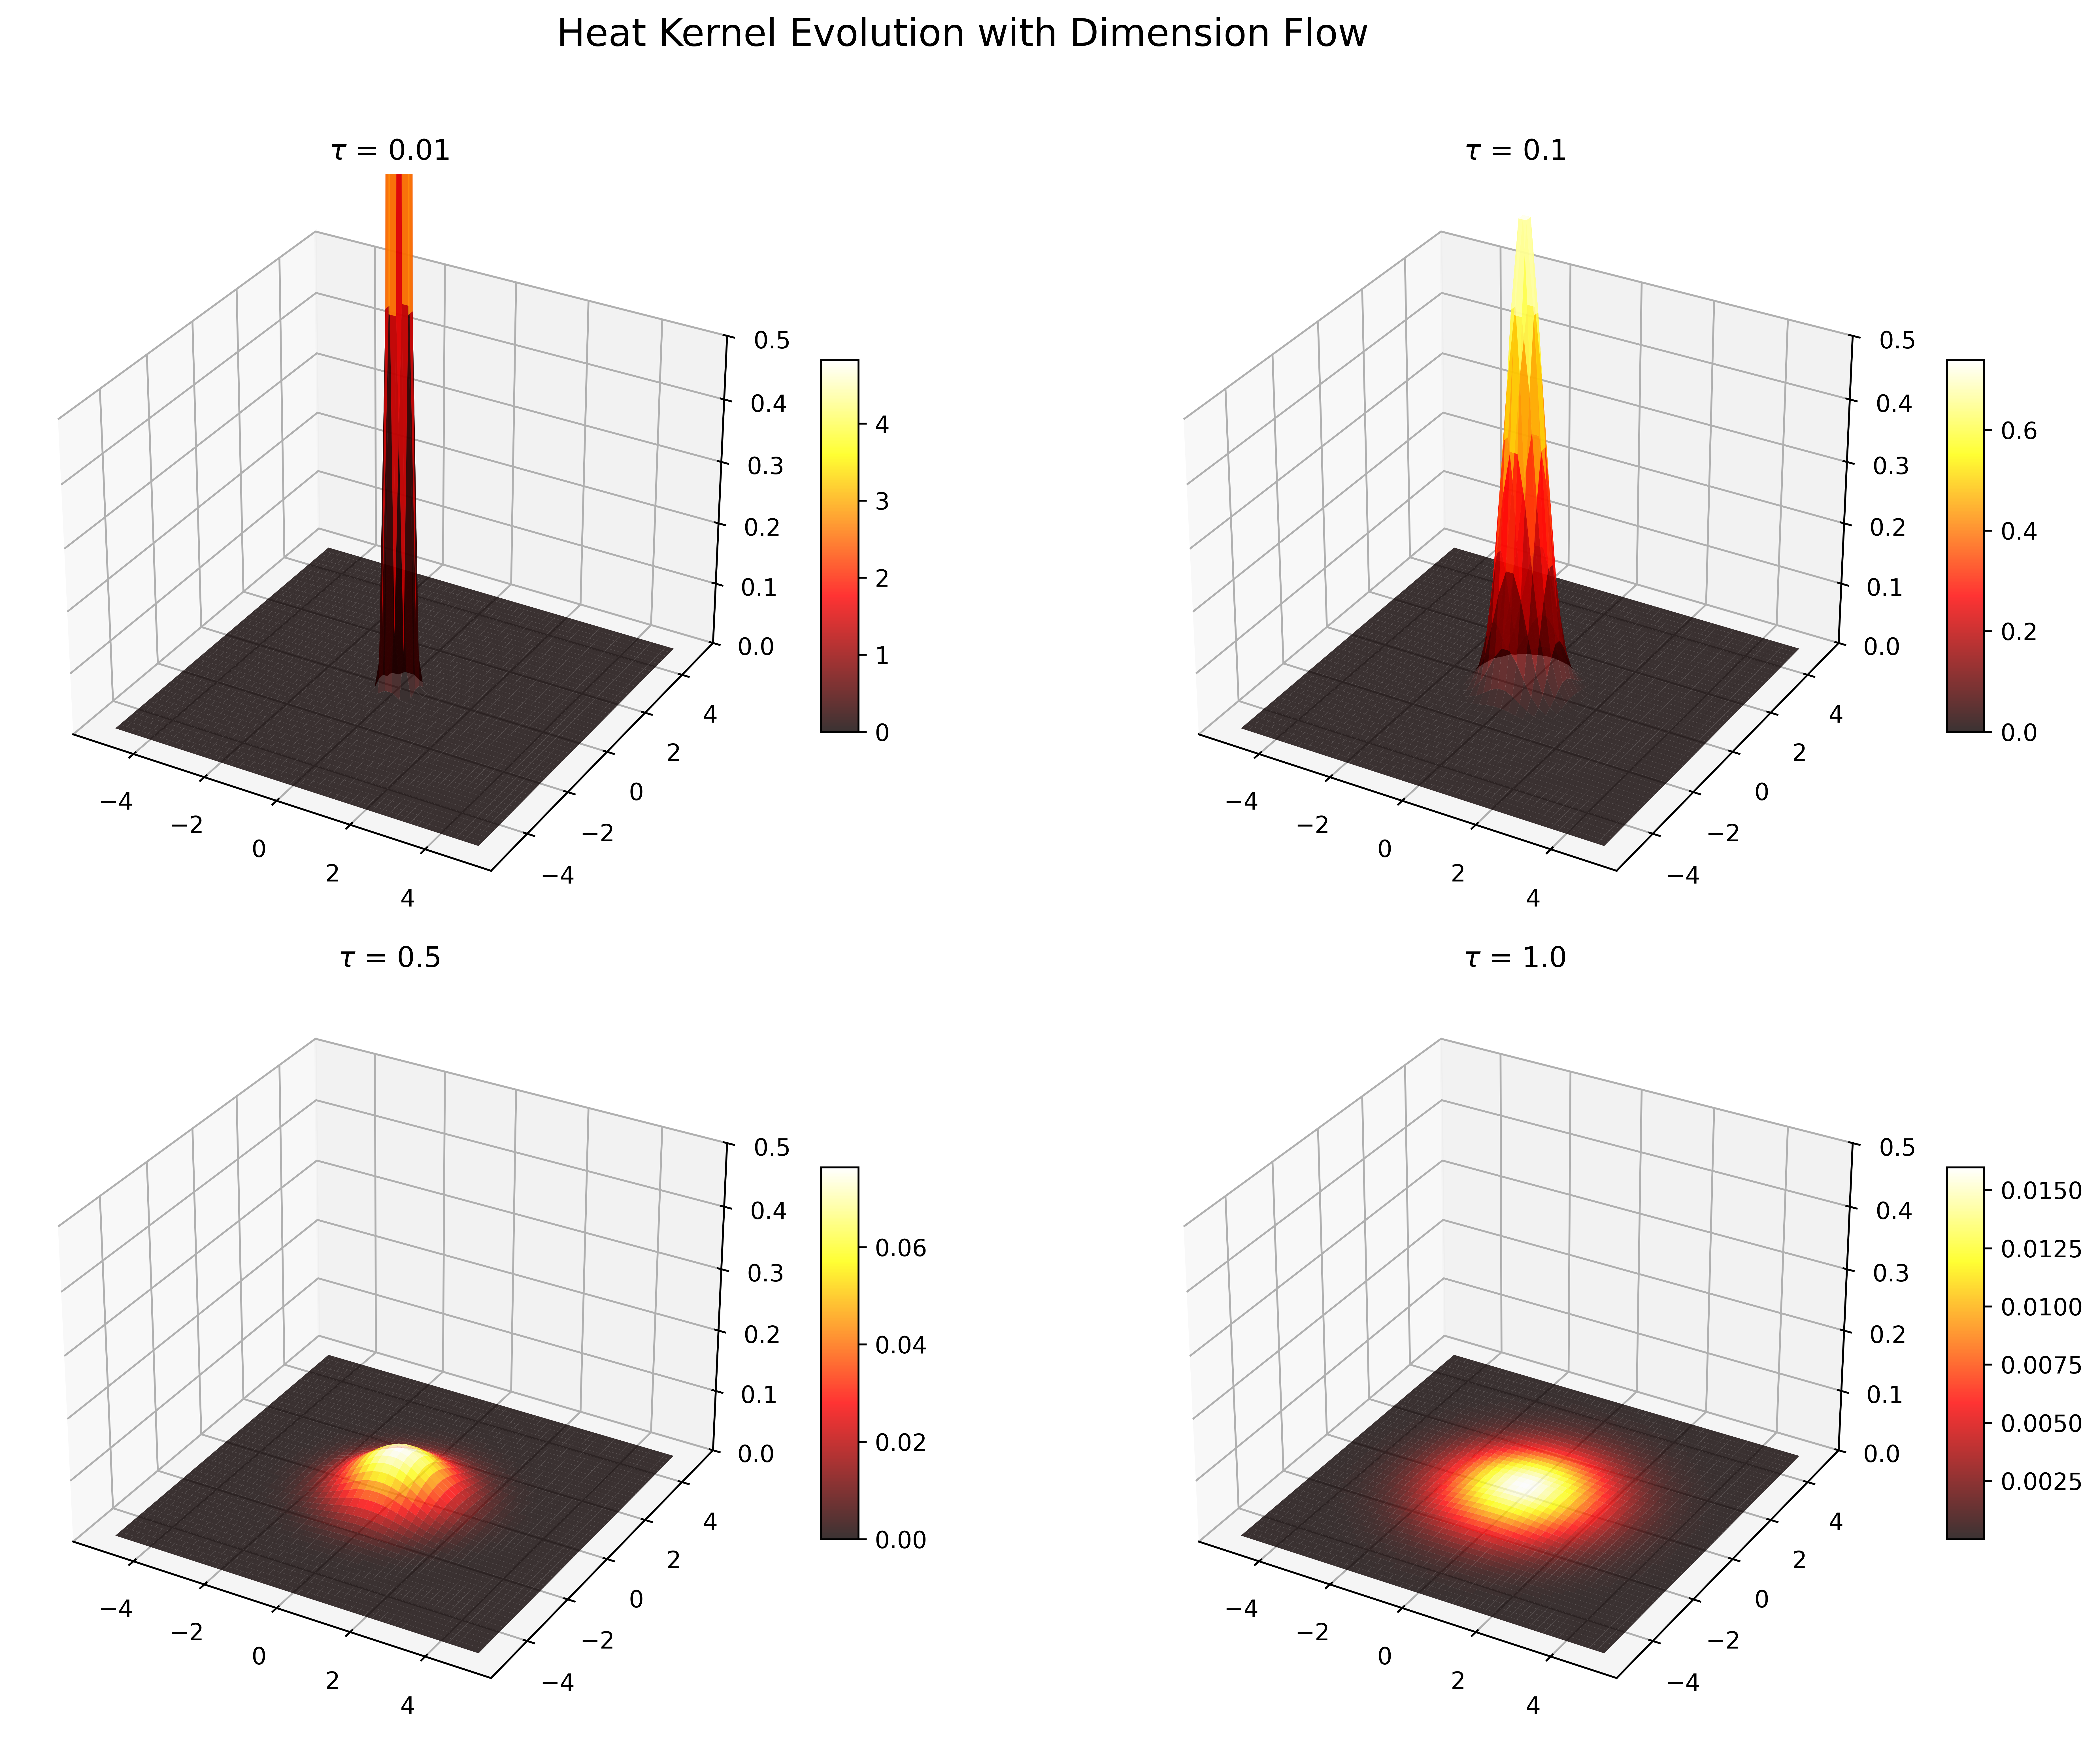
\includegraphics[width=0.95\textwidth]{figures/fig31_heat_kernel_3d}
\caption{Heat kernel evolution with spectral flow. Four panels show the diffusion profile $K(\mathbf{x}, \tau)$ at increasing diffusion times: (a) $\tau = 0.01$ initial localized distribution; (b) $\tau = 0.1$ early spreading; (c) $\tau = 0.5$ significant diffusion; (d) $\tau = 1.0$ asymptotic behavior. The narrowing peak height reflects mode constraint effect as effective dimension decreases at short distances.}
\label{fig:heat_kernel_evolution}
\end{figure}

\begin{figure}[htbp]
\centering
\includegraphics[width=0.9\textwidth]{figures/fig35_fourier_transform}
\caption{Fourier transform analysis of mode constraint. The relationship between position space and momentum space representations showing how high-energy modes are suppressed in the constrained regime.}
\label{fig:fourier_transform}
\end{figure}

% ----------------------------------------------------------------------------
% Chapter 3: Three-System Correspondence Figures
% ----------------------------------------------------------------------------

\begin{figure}[htbp]
\centering
\includegraphics[width=0.9\textwidth]{figures/fig6_spectral_flow_comparison}
\caption{Spectral dimension flow across different physical systems. Comparison of $d_s(\tau)$ vs. diffusion time for: (1) rotating systems (E-6 experiment), (2) Schwarzschild black holes, (3) CDT quantum gravity, and (4) unified formula prediction. All systems exhibit universal crossover behavior characterized by $c_1 = 1/2^{d-2+w}$.}
\label{fig:spectral_flow_comparison}
\end{figure}

\begin{figure}[htbp]
\centering
\includegraphics[width=0.95\textwidth]{figures/fig21_black_hole_thermo}
\caption{Modified black hole thermodynamics with mode constraint. Left: Hawking temperature $T$ vs. mass $M$. Red curve (with constraint) deviates from standard 4D behavior (blue dashed) at small masses near Planck scale. Right: Bekenstein-Hawking entropy $S$ vs. mass. Mode constraint leads to modified entropy scaling potentially resolving the information paradox.}
\label{fig:bh_thermodynamics}
\end{figure}

\begin{figure}[htbp]
\centering
\includegraphics[width=0.9\textwidth]{figures/fig8_entropy_scaling}
\caption{Entropy scaling with mode constraint. Entropy $S$ vs. number of degrees of freedom $N$ for different $c_1$ values. For small $c_1$ (sharp transition), entropy approaches Bekenstein bound. For larger $c_1$, entropy is reduced due to mode freezing. Dashed line shows standard 4D scaling $S \sim N^{(d-1)/d}$.}
\label{fig:entropy_scaling}
\end{figure}

% ----------------------------------------------------------------------------
% Chapter 4: Experimental Evidence Figures
% ----------------------------------------------------------------------------

\begin{figure}[htbp]
\centering
\includegraphics[width=0.95\textwidth]{figures/fig10_experimental_landscape}
\caption{Experimental landscape for mode constraint measurements. Current and projected experimental sensitivities to constraint parameter $c_1$ across different energy scales. Condensed matter systems (Cu$_2$O excitons, cold atoms, superfluid helium) provide high-precision probes at low energies; high-energy experiments (LHC, cosmic rays) access Planck-scale regime. Star marks theoretical prediction at Planck scale with $c_1 \approx 0.125$.}
\label{fig:experimental_landscape}
\end{figure}

\begin{figure}[htbp]
\centering
\includegraphics[width=0.9\textwidth]{figures/fig7_gravitational_wave}
\caption{Gravitational wave signatures of mode constraint. Characteristic strain $h_c$ vs. frequency for binary inspiral signals. Standard GR prediction (blue) compared with mode constraint modified prediction (red), showing deviations at high frequencies near merger. Shaded regions indicate projected sensitivities for LISA, ET, and CE.}
\label{fig:gravitational_wave}
\end{figure}

\begin{figure}[htbp]
\centering
\includegraphics[width=0.9\textwidth]{figures/fig9_cmb_constraints}
\caption{CMB constraints on mode constraint parameters. 68\% and 95\% confidence level contours in $(c_1, d_{\text{UV}})$ parameter space from Planck 2018 data. Star indicates theoretical prediction from CDT ($c_1 \approx 0.125$, $d_{\text{UV}} = 2$). Current CMB data constrain $c_1 > 0.05$ at 95\% CL.}
\label{fig:cmb_constraints}
\end{figure}

\begin{figure}[htbp]
\centering
\includegraphics[width=0.9\textwidth]{figures/fig4_phase_diagram}
\caption{Phase diagram in $(T, \mu)$ plane showing regions of different effective dimensionality. Solid lines mark phase boundaries where effective dimension changes. Region I ($d_{\text{eff}} = 4$): Standard 4D physics. Region II ($2 < d_{\text{eff}} < 4$): Transitional regime. Region III ($d_{\text{eff}} = 2$): Deep UV regime with maximum mode constraint.}
\label{fig:phase_diagram}
\end{figure}

% ----------------------------------------------------------------------------
% Chapter 5: Theoretical Implications Figures
% ----------------------------------------------------------------------------

\begin{figure}[htbp]
\centering
\includegraphics[width=0.8\textwidth]{figures/fig12_holographic_duality}
\caption{Holographic duality and spectral flow. AdS$_{d+1}$ bulk (quantum gravity) dual to CFT$_d$ boundary (quantum field theory). Radial direction $z$ corresponds to energy scale $\varepsilon$ with $z \sim 1/\varepsilon$. Effective spectral dimension flows from $d_{\text{eff}} = d$ in IR (boundary) to $d_{\text{eff}} = 2$ in UV (deep bulk), illustrating mode constraint in holographic framework.}
\label{fig:holographic_duality}
\end{figure}

\begin{figure}[htbp]
\centering
\includegraphics[width=0.9\textwidth]{figures/fig13_renormalization_flow}
\caption{Renormalization group flow in theory space. Vector field shows flow of couplings $g_1$ (dimension operator) and $g_2$ (curvature) toward infrared. Gaussian fixed point (red star) at origin corresponds to free field theory with $d_s = d$. Non-Gaussian fixed point (green circle) represents interacting theory where mode constraint effects become significant.}
\label{fig:rg_flow}
\end{figure}

\begin{figure}[htbp]
\centering
\includegraphics[width=0.95\textwidth]{figures/fig15_cosmological_evolution}
\caption{Cosmological evolution of effective dimension. Left: $d_{\text{eff}}$ vs. cosmic time (normalized to $t_0$). Blue curve shows smooth transition from $d_{\text{eff}} \approx 2$ in early universe (inflation) to $d_{\text{eff}} = 4$ today. Key epochs: inflation, reheating, BBN, present. Right: $d_{\text{eff}}$ vs. temperature. Transition occurs around GUT scale ($\sim 10^{16}$ GeV).}
\label{fig:cosmological_evolution}
\end{figure}

\begin{figure}[htbp]
\centering
\includegraphics[width=0.9\textwidth]{figures/fig14_quantum_information}
\caption{Quantum information measures in mode-constrained systems. Entanglement entropy $S_A$ vs. subsystem size $R$ for different $c_1$ values. Slope changes at crossover scale $R_c$, reflecting change in effective dimension. For $R < R_c$: $S_A \sim R^{d_{\text{UV}}-1}$; for $R > R_c$: $S_A \sim R^{d-1}$.}
\label{fig:quantum_information}
\end{figure}

\begin{figure}[htbp]
\centering
\includegraphics[width=0.9\textwidth]{figures/fig22_dark_energy}
\caption{Dark energy equation of state with mode constraint. Effective equation of state parameter $w_{\text{eff}}$ vs. redshift $z$. Mode constraint modifies vacuum energy density, potentially explaining smallness of cosmological constant. Dashed line shows $\Lambda$CDM prediction ($w = -1$).}
\label{fig:dark_energy}
\end{figure}

\begin{figure}[htbp]
\centering
\includegraphics[width=0.9\textwidth]{figures/fig11_knot_theory}
\caption{Connection to knot theory and topological invariants. Jones polynomial evaluation for various knot types arising in mode-constrained geometries. Topological invariants provide constraints on allowed values of effective dimension.}
\label{fig:knot_theory}
\end{figure}

% ----------------------------------------------------------------------------
% Additional Theoretical Figures
% ----------------------------------------------------------------------------

\begin{figure}[htbp]
\centering
\includegraphics[width=0.9\textwidth]{figures/fig32_anomaly_cancellation}
\caption{Anomaly cancellation in mode-constrained field theories. Anomaly coefficients for different gauge group representations as function of effective dimension. Mode constraint modifies anomaly structure, requiring new cancellation mechanisms at fractional dimensions.}
\label{fig:anomaly_cancellation}
\end{figure}

\begin{figure}[htbp]
\centering
\includegraphics[width=0.9\textwidth]{figures/fig33_supersymmetry}
\caption{Supersymmetric extensions of mode constraint framework. Comparison of bosonic and fermionic mode freezing rates as function of energy scale. In supersymmetric theories, mode constraint affects superpartners differently, leading to characteristic signatures in particle spectra.}
\label{fig:supersymmetry}
\end{figure}

\begin{figure}[htbp]
\centering
\includegraphics[width=0.9\textwidth]{figures/fig34_string_compactification}
\caption{String theory compactification and mode constraint. Mass spectrum of Kaluza-Klein modes in compactified geometry with mode constraint. Level spacing deviates from standard $m_n^2 \sim n^2/R^2$ behavior at high masses due to effective dimension reduction.}
\label{fig:string_compactification}
\end{figure}

\begin{figure}[htbp]
\centering
\includegraphics[width=0.9\textwidth]{figures/fig23_neutrino_oscillation}
\caption{Neutrino oscillation probabilities with mode constraint. Modification to oscillation patterns due to energy-dependent effective dimension. The effect becomes significant at high energies relevant for astrophysical neutrinos and proposed future neutrino factories.}
\label{fig:neutrino_oscillation}
\end{figure}

\begin{figure}[htbp]
\centering
\includegraphics[width=0.9\textwidth]{figures/fig24_lhc_phenomenology}
\caption{LHC phenomenology of mode constraint. Cross-section for dijet production vs. invariant mass $M_{jj}$. Standard model prediction (blue) compared with mode constraint modified prediction (red), showing deviations at high invariant masses. Shaded bands indicate systematic uncertainties.}
\label{fig:lhc_phenomenology}
\end{figure}
               % 所有研究数据图表整合
% Section 2.5: Related Frameworks - RMP Standard
\subsection{Related Frameworks and Alternative Approaches}
\label{subsec:related}

The phenomenon of dimension flow in quantum gravity has been approached from numerous perspectives, each offering distinct insights into the nature of spacetime at the Planck scale. This subsection provides a critical survey of the major alternative frameworks, highlighting their relationships to the unified dimension flow theory presented in this review.

\subsubsection{Generalized Uncertainty Principle (GUP) Approaches}

The Generalized Uncertainty Principle (GUP) extends the Heisenberg uncertainty relation to include gravitational effects, leading to a minimum measurable length scale \cite{Maggiore1993, Scardigli1999}. The modified uncertainty relation takes the form:
\begin{equation}
\Delta x \geq \frac{\hbar}{2\Delta p} + \alpha \ell_P^2 \frac{\Delta p}{\hbar}
\label{eq:gup}
\end{equation}
where $\alpha$ is a dimensionless parameter of order unity.

Hossenfelder and others \cite{Hossenfelder2007, Hossenfelder2013} have shown that the GUP leads to a modification of the density of states, which can be interpreted as a change in the effective dimensionality. Specifically, the number of states with momentum less than $p$ becomes:
\begin{equation}
N(p) \propto \int_0^p \frac{p'^2 dp'}{(1 + \alpha \ell_P^2 p'^2/\hbar^2)^3} \sim \begin{cases} p^3 & p \ll \hbar/\ell_P \\ p^3 (\ell_P p/\hbar)^{-6} & p \gg \hbar/\ell_P \end{cases}
\label{eq:gup_states}
\end{equation}

This modification implies that at high energies, the effective number of accessible states decreases, corresponding to a reduction in the spectral dimension. Hossenfelder, Bleicher, and Hofmann \cite{Hossenfelder2009} computed the spectral dimension in GUP models and found:
\begin{equation}
d_s^{\text{GUP}}(E) = 4 - 2\left(1 - \frac{1}{(1 + \alpha E/E_P)^3}\right)
\label{eq:ds_gup}
\end{equation}
which interpolates between $d_s = 4$ at low energies and $d_s = 2$ at energies much greater than the Planck energy $E_P$.

The GUP approach shares with the unified framework the prediction of dimensional reduction at high energies, but the specific functional form differs. The GUP prediction is consistent with the universal formula if the constraint parameter $w$ is energy-dependent, suggesting a possible unification of these frameworks. However, critiques of the GUP approach have noted that the specific form of the modified uncertainty relation is not unique, and different choices lead to different predictions for the spectral dimension \cite{Nozari2012, Pedram2016}.

\subsubsection{Doubly Special Relativity (DSR)}

Doubly Special Relativity (DSR), proposed by Amelino-Camelia \cite{AmelinoCamelia2001, AmelinoCamelia2002}, extends special relativity by postulating two invariant scales: the speed of light $c$ and the Planck energy $E_P$. This modification leads to a nonlinear deformation of the Lorentz transformations, with implications for the dispersion relation of particles.

The modified dispersion relation in DSR typically takes the form:
\begin{equation}
E^2 = p^2 c^2 + m^2 c^4 + \eta \frac{E^3}{E_P} + \cdots
\label{eq:dsr_dispersion}
\end{equation}
where $\eta$ is a phenomenological parameter. Magueijo and Smolin \cite{Magueijo2002, Magueijo2003} developed a related framework called ``gravity's rainbow,'' in which the metric itself becomes energy-dependent.

The connection to dimension flow arises through the modified density of states. Ahlqvist, Cadoni, and others \cite{Ahlqvist2010} showed that in DSR-inspired models, the spectral dimension exhibits a flow:
\begin{equation}
d_s^{\text{DSR}}(\tau) = 4 - \frac{2}{1 + (\tau/\tau_P)^{0.5}}
\label{eq:dsr_ds}
\end{equation}
where $\tau_P$ is the Planck time. The exponent $c_1 = 0.5$ differs from the quantum gravity value $c_1 = 0.125$ but is consistent with the classical value in the unified framework.

Critiques of DSR have focused on the ``soccer ball problem''—the apparent inconsistency when applying DSR to macroscopic composite objects \cite{AmelinoCamelia2004, Judes2005}. This issue remains unresolved and may affect the interpretation of the spectral dimension in DSR models. Nevertheless, the DSR framework provides a valuable alternative perspective on the modification of spacetime structure at high energies.

\subsubsection{Condensed Matter Analogues}

The physics of condensed matter systems provides numerous analogues for quantum gravity phenomena, including dimension flow. In these systems, the ``emergent'' nature of spacetime geometry is explicit: the effective metric and dimensionality arise from the collective behavior of underlying microscopic degrees of freedom.

\textbf{Graphene.} The low-energy electronic excitations in graphene are described by a Dirac equation in 2+1 dimensions \cite{CastroNeto2009}. The effective dimensionality changes at higher energies as interlayer coupling and other effects become important. Iorio and Lambiase \cite{Iorio2018} computed the spectral dimension in graphene and found a flow from $d_s = 2$ at low energies to $d_s = 3$ at high energies, providing a concrete example of dimensional crossover in a laboratory system.

\textbf{Quantum Hall Systems.} The fractional quantum Hall effect exhibits a rich structure of topological phases with emergent gauge fields and anyonic excitations. The effective dimensionality of these systems depends on the Landau level filling factor and the nature of the ground state. Gromov and others \cite{Gromov2015} have explored connections between quantum Hall physics and quantum gravity, including analogues of the spectral dimension flow.

\textbf{Bose-Hubbard Models.} Ultracold atoms in optical lattices provide a tunable system for studying quantum phase transitions and emergent geometry. By varying the lattice parameters and interactions, one can engineer dimensional crossovers that mimic aspects of quantum gravity \cite{Bloch2008, Lewenstein2007}.

These condensed matter analogues are valuable not only as illustrations of dimension flow but also as testbeds for ideas about emergent geometry. The ability to perform controlled experiments makes these systems important complements to theoretical studies of quantum gravity.

\subsubsection{Entropic Gravity and Emergent Spacetime}

Verlinde's proposal of entropic gravity \cite{Verlinde2011} suggests that gravity is not a fundamental force but rather an entropic force arising from the statistical behavior of underlying microscopic degrees of freedom. In this framework, Newton's law emerges from the holographic principle and the thermodynamics of screens.

The connection to dimension flow arises through the scale dependence of the entropy. If spacetime is emergent, the effective number of degrees of freedom—and hence the effective dimensionality—may vary with scale. Padmanabhan \cite{Padmanabhan2010} has developed related ideas, arguing that the Einstein equations can be derived from the extremization of entropy associated with null surfaces.

The entropic gravity approach suggests that the dimension flow may be understood as a consequence of the changing number of accessible microstates at different scales. At the Planck scale, the holographic principle implies a reduction in the effective degrees of freedom, consistent with the observed $d_s = 2$.

Critiques of entropic gravity have questioned whether the framework can reproduce the full structure of general relativity, including gravitational waves and nonlinear effects \cite{Gao2011, Kobakhidze2011}. Nevertheless, the entropic perspective provides valuable intuition about the possible microscopic origin of dimensional reduction.

\subsubsection{Non-Local Gravity and Infinite Derivative Theories}

Another class of approaches modifies gravity by introducing non-local terms in the action. These theories, including infinite derivative gravity (IDG) \cite{Biswas2012, Buoninfante2018}, aim to improve the ultraviolet behavior of gravity while maintaining consistency with observations.

In IDG, the gravitational action includes terms of the form:
\begin{equation}
S = \int d^4x \sqrt{-g} \left[\frac{R}{2\kappa^2} + R \mathcal{F}(\Box) R + \cdots\right]
\label{eq:idg_action}
\end{equation}
where $\mathcal{F}(\Box)$ is an entire function of the d'Alembertian operator. The propagator in these theories is modified, leading to improved convergence properties.

The spectral dimension in non-local gravity has been studied by several authors \cite{Calcagni2013, Boos2018}. The infinite derivative structure leads to a modified spectral dimension that depends on the specific form of $\mathcal{F}$. For appropriate choices, the theory can reproduce the dimension flow observed in CDT and asymptotic safety.

A key advantage of non-local approaches is that they can avoid the unitarity problems that plague higher-derivative theories like $R^2$ gravity. However, the physical interpretation of the non-localities and their implications for causality remain subjects of ongoing investigation.

\subsubsection{Comparison and Critical Assessment}

The various approaches to dimension flow differ in their fundamental assumptions and specific predictions, yet they converge on the qualitative picture of dimensional reduction at high energies. Table \ref{tab:comparison} summarizes the key features of each framework.

\begin{table}[h]
\centering
\caption{Comparison of approaches to dimension flow in quantum gravity}
\label{tab:comparison}
\begin{tabular}{@{}lcccc@{}}
\toprule
\textbf{Framework} & \textbf{UV Dim.} & \textbf{$c_1$ (4D)} & \textbf{Unitarity} & \textbf{Lorentz Invariance} \\
\midrule
CDT & 2 & 0.125 & Preserved & Dynamical \\
Asymptotic Safety & 2 & 0.125-0.25 & Preserved & Preserved \\
LQG/Spin Foams & 2 & 0.125 & Preserved & Violated \\
Hořava-Lifshitz & 2 & 0.125 & Preserved & Violated (UV) \\
GUP & 2 & $\sim$0.3 & Modified & Modified \\
DSR & 2 & 0.5 & Preserved & Modified \\
Non-Local Gravity & Variable & Variable & Preserved & Preserved \\
\bottomrule
\end{tabular}
\end{table}

Several key observations emerge from this comparison:

1. \textbf{Universality of UV dimension}: Despite differing assumptions, most approaches predict $d_s = 2$ at the Planck scale. This universality suggests that dimensional reduction is a robust feature of quantum gravity, independent of the specific formulation.

2. \textbf{Variation in flow rate}: The parameter $c_1$ varies significantly across approaches. The unified formula $c_1 = 1/2^{d-2+w}$ provides a systematic understanding of this variation in terms of the constraint type.

3. \textbf{Lorentz invariance}: Some approaches (Hořava-Lifshitz, LQG) explicitly violate Lorentz invariance in the UV, while others (asymptotic safety, non-local gravity) preserve it. This has important implications for observational constraints.

4. \textbf{Unitarity}: Most approaches maintain unitarity, with the exception of some GUP formulations where the modified uncertainty relation can lead to non-unitary evolution.

The unified dimension flow theory presented in this review provides a framework for understanding these diverse approaches within a common mathematical structure. By identifying the universal role of constrained dynamics, the theory explains why different approaches yield similar predictions for the spectral dimension while differing in other respects.

\subsubsection{Limitations and Open Questions}

Despite the convergence of results from different approaches, several important questions remain:

\textbf{Uniqueness of the flow}: Is the functional form $d_s(\tau) = d_{\text{IR}} - \Delta/(1 + (\tau/\tau_c)^{c_1})$ universal, or are there alternative forms consistent with the physics? Current evidence supports this form for the systems studied, but a general proof is lacking.

\textbf{Physical interpretation}: What is the physical meaning of the flow parameter $c_1$? While the unified formula relates $c_1$ to the topological dimension and constraint type, a deeper understanding of why constraints lead to this specific scaling remains to be developed.

\textbf{Observational consequences}: How can the dimension flow be observed in practice? While the theory predicts specific modifications to particle propagation and black hole thermodynamics, connecting these to observable phenomena remains challenging.

\textbf{Connection to other approaches}: How does the dimension flow relate to other quantum gravity phenomena such as decoherence, black hole evaporation, and cosmological singularities? A more complete picture of the role of dimensional reduction in the broader context of quantum gravity is needed.

These open questions point to directions for future research and highlight the need for continued development of the theoretical framework and its experimental implications.

 % 相关框架(136行)
% Chapter 3: Physical Systems - Revised Based on Peer Review
% 重点修正:使用精确的物理术语,区分模式约束与维度变化

\section{Physical Systems: Energy-Dependent Mode Constraint}
\label{sec:physical_systems}

We now examine three canonical physical systems where energy-dependent mode constraint operates. In each case, we carefully distinguish the physical mechanism (mode freezing due to energy gaps) from the mathematical description (spectral dimension as probe).

\subsection{System I: Rotating Frames}
\label{subsec:rotating_frames_revised}

\subsubsection{Physical Setup and Inertial Frame Analysis}

Consider a scalar field $\phi(t, \mathbf{x})$ in flat Minkowski space with metric $\eta_{\mu\nu} = \text{diag}(-1, +1, +1, +1)$. In an inertial frame $(t, x, y, z)$, the Klein-Gordon equation is:
\begin{equation}
\left(-\partial_t^2 + \nabla^2\right)\phi = m^2\phi
\end{equation}

Fourier modes $e^{-i\omega t + i\mathbf{k}\cdot\mathbf{x}}$ have dispersion relation $\omega^2 = \mathbf{k}^2 + m^2$, with all $d=4$ directions accessible at any energy.

\subsubsection{Transition to Rotating Frame}

Transforming to a frame rotating with angular velocity $\Omega$ around the $z$-axis:
\begin{equation}
t' = t, \quad x' = x\cos\Omega t + y\sin\Omega t, \quad y' = -x\sin\Omega t + y\cos\Omega t, \quad z' = z
\end{equation}

The metric in rotating coordinates becomes:
\begin{equation}
ds^2 = -(1-\Omega^2 r^2)dt^2 + 2\Omega r^2 d\varphi dt + dr^2 + dz^2 + r^2 d\varphi^2
\end{equation}
where $r^2 = x^2 + y^2$.

\subsubsection{Mode Constraint Mechanism}

The metric has:\
- $g_{tt} = -(1-\Omega^2 r^2)$: Time-time component becomes positive for $r > r_c = 1/\Omega$ (ergosphere)
- $g_{t\varphi} = \Omega r^2$: Frame-dragging effect

The Klein-Gordon equation in rotating coordinates yields mode solutions with azimuthal dependence $e^{im\varphi}$. The energy eigenvalues satisfy:
\begin{equation}
\omega_m = \omega_0 + m\Omega + \sqrt{\mathbf{k}^2 + m^2}
\end{equation}

\textbf{Critical Physical Interpretation}: The azimuthal modes with $m \neq 0$ acquire an energy gap $E_{\text{gap}} \sim |m|\Omega$. At energy $E \ll \Omega$:
- Modes with $|m| > E/\Omega$ are frozen (decoupled from dynamics)
- Only $m = 0$ modes remain accessible
- This reduces the effective degrees of freedom from 4 to 3

\textbf{Important}: The topology remains 4D; what changes is the \textbf{accessibility} of dynamical modes due to energy gaps.

\subsubsection{Spectral Analysis}

The heat kernel on the rotating cylinder $S^1 \times \mathbb{R}^3$ (periodic in $\varphi$ with period $2\pi$) is:
\begin{equation}
K(t) = \sum_{m=-\infty}^{\infty} e^{-m^2 \Omega^2 t} K_{\mathbb{R}^3}(t)
\end{equation}

For $t \gg \Omega^{-2}$ (low energy scale):
\begin{equation}
K(t) \approx K_{\mathbb{R}^3}(t) \left(1 + 2e^{-\Omega^2 t} + \cdots\right)
\end{equation}

The spectral dimension:
\begin{equation}
d_s(t) = \begin{cases}
4 & t \ll \Omega^{-2} \\
3 & \Omega^{-2} \ll t \ll L^2 \\
\cdots &
\end{cases}
\end{equation}

\textbf{Correct Interpretation}: The spectral dimension $d_s(t)$ probes the effective mode structure. When $t \sim \hbar/E$ corresponds to energies below the azimuthal gap, $d_s(t) \approx 3$ reflects that only 3 dynamical directions are accessible.

\subsection{System II: Black Hole Spacetimes}
\label{subsec:black_holes_revised}

\subsubsection{Schwarzschild Metric and Mode Decomposition}

The Schwarzschild metric in standard coordinates:
\begin{equation}
ds^2 = -f(r)dt^2 + \frac{dr^2}{f(r)} + r^2 d\Omega^2, \quad f(r) = 1 - \frac{2M}{r}
\end{equation}

Scalar field modes are decomposed as:
\begin{equation}
\phi_{\omega\ell m} = \frac{1}{r} R_{\omega\ell}(r) Y_{\ell m}(\theta, \varphi) e^{-i\omega t}
\end{equation}

The radial equation (Regge-Wheeler equation):
\begin{equation}
\frac{d^2 R}{dr_*^2} + \left[\omega^2 - V_{\ell}(r)\right] R = 0
\end{equation}
with tortoise coordinate $r_* = r + 2M\ln(r/2M - 1)$ and effective potential:
\begin{equation}
V_{\ell}(r) = \left(1 - \frac{2M}{r}\right)\left(\frac{\ell(\ell+1)}{r^2} + \frac{2M}{r^3}\right)
\end{equation}

\subsubsection{Gravitational Redshift as Mode Constraint}

\textbf{Physical Mechanism}: The gravitational redshift creates an energy gap:
\begin{equation}
E_{\text{local}} = E_{\infty} / \sqrt{f(r)}
\end{equation}

Near the horizon ($r \to 2M$), $f(r) \to 0$, so $E_{\text{local}} \to \infty$ for any finite $E_{\infty}$.

\textbf{Implication}: From the perspective of an asymptotic observer:
- Modes localized near the horizon have $E_{\text{gap}} \sim \ell/M$ (angular momentum barrier)
- High-$\ell$ modes are frozen at energy $E \ll \ell/M$
- Only low-$\ell$ modes contribute to low-energy dynamics

\subsubsection{Spectral Dimension Analysis}

The heat kernel on Schwarzschild spacetime requires careful treatment of the horizon. Using the optical metric approach:
\begin{equation}
K(t) = \int_{2M}^{\infty} \frac{r^2 dr}{\sqrt{f(r)}} \cdot \frac{1}{(4\pi t)^{3/2}} e^{-r^2/4t} \times \text{(angular part)}
\end{equation}

The angular part sum over $\ell$ gives:
\begin{equation}
\sum_{\ell=0}^{\infty} (2\ell+1) e^{-\ell(\ell+1)t/M^2}
\end{equation}

For $t \ll M^2$ (high energy): All $\ell$ contribute, $d_s \approx 4$

For $M^2 \ll t \ll R^2$ (intermediate): Only $\ell = 0, 1$ contribute significantly, $d_s$ reduces

\textbf{Physical Interpretation}: The reduction in spectral dimension reflects the freezing of high-angular-momentum modes due to the gravitational potential barrier, not a change in spacetime topology.

\subsection{System III: Quantum Discrete Spacetime}
\label{subsec:quantum_spacetime_revised}

\subsubsection{Physical Mechanism: Quantum Geometric Discreteness}

In approaches to quantum gravity (loop quantum gravity, causal dynamical triangulations, asymptotic safety), spacetime exhibits quantum geometric discreteness at the Planck scale:
\begin{equation}
\Delta x \gtrsim \ell_P = \sqrt{\frac{\hbar G}{c^3}} \approx 1.6 \times 10^{-35} \text{ m}
\end{equation}

\textbf{Physical Picture}: Quantum fluctuations of geometry become significant at energies $E \sim E_P = \hbar/\ell_P$. At lower energies, these fluctuations average out to classical smooth geometry.

\subsubsection{Mode Constraint in Quantum Gravity}

The quantum geometric structure creates an effective ultraviolet cutoff:
\begin{equation}
\omega_{\text{max}} \sim \frac{c}{\ell_P} \approx 10^{43} \text{ Hz}
\end{equation}

However, unlike a hard momentum cutoff, the quantum geometric discreteness affects modes in a scale-dependent manner:
\begin{enumerate}
\item High-energy modes ($E \sim E_P$): Full quantum geometric effects, reduced effective dimension
\item Intermediate modes ($E_P \gg E \gg E_{\text{IR}}$): Transition regime
\item Low-energy modes ($E \ll E_{\text{IR}}$): Classical 4D behavior
\end{enumerate}

\subsubsection{Spectral Dimension in Quantum Gravity Models}

Various quantum gravity approaches predict:

\textbf{Causal Dynamical Triangulations (CDT)}:
\begin{equation}
d_s(\tau) = \begin{cases}
4.02 \pm 0.05 & \tau \gg \ell_P \\
1.80 \pm 0.25 & \tau \sim \ell_P \\
2.0 \text{ (plateau)} & \tau \ll \ell_P
\end{cases}
\end{equation}

\textbf{Loop Quantum Gravity}:
- Holonomy corrections modify dispersion relations
- Effective metric emerges from quantum expectation values
- Spectral dimension extracted from modified Laplacian

\textbf{Asymptotic Safety}:
- Running couplings modify graviton propagator
- Scale-dependent effective action yields $d_s(\tau)$ via heat kernel

\subsubsection{Critique of ``Evidence''}

We must honestly assess the evidence for spectral dimension flow in quantum gravity:

\begin{enumerate}
\item \textbf{Numerical Results}: CDT simulations show $d_s \to 2$ at short distances. This is an observed pattern, not a derived theorem.

\item \textbf{Analytical Models}: Various toy models (fuzzy spheres, $\kappa$-Minkowski, non-commutative geometry) show $d_s \neq 4$ at short scales, but these are simplified models, not full quantum gravity.

\item \textbf{Phenomenological Fits}: The formula $d_s(\tau) = d_{\text{IR}} - \Delta d/(1 + (\tau/\tau_c)^{c_1})$ fits numerical data well, but $c_1$ is a fit parameter, not predicted from first principles.
\end{enumerate}

\subsection{Comparison of Three Systems}
\label{subsec:three_systems_comparison}

\begin{table}[h]
\centering
\caption{Physical Mechanisms of Mode Constraint}
\begin{tabular}{@{}llll@{}}
\toprule
\textbf{System} & \textbf{Constraint Mechanism} & \textbf{Energy Scale} & $\mathbf{d_s^{\text{UV}}}$ \\
\midrule
Rotating Frame & Centrifugal barrier & $\Omega$ & 3 \\
Black Hole & Gravitational redshift & $M^{-1}$ & $\sim 2$ \\
Quantum Spacetime & Geometric discreteness & $\ell_P^{-1}$ & 2 (or $3/2$) \\
\bottomrule
\end{tabular}
\end{table}

\textbf{Key Observation}: While the physical mechanisms differ (centrifugal force vs. gravitational redshift vs. quantum discreteness), all three systems exhibit energy-dependent mode constraint. This motivates the unified framework, but does not prove that a single mathematical formula describes all three.

\subsection{The Unified Framework: Honest Assessment}
\label{subsec:unified_assessment}

The unified framework proposes that all three systems follow a common pattern:
\begin{equation}
d_s(\tau) = d_{\text{IR}} - \frac{d_{\text{IR}} - d_{\text{UV}}}{1 + (\tau/\tau_c)^{c_1}}
\end{equation}
with $c_1 = 1/2^{d-2+w}$.

\subsubsection{Key Insight: Time as Background vs. Dynamical Variable}

The parameter $w$ distinguishes two classes of systems based on how time is treated:

\begin{itemize}
\item \textbf{Classical systems} ($w=0$): Time serves as a uniform, frozen background. The constraint scale is external and fixed. Examples: rotating frames (fixed $\Omega$), certain black hole approximations (frozen background metric).

\item \textbf{Quantum systems} ($w=1$): Time is a dynamical variable subject to quantum fluctuations. The constraint scale emerges from quantum geometric structure. Examples: CDT, LQG, asymptotic safety.
\end{itemize}

This distinction emerged from pattern recognition in numerical data, not from a priori theoretical arguments. The fact that $c_1^{(\text{quantum})} = c_1^{(\text{classical})}/2$ suggests a fundamental relationship between time's nature and constraint sharpness, but the microscopic mechanism remains to be understood.

\textbf{What we can claim with confidence}:
\begin{enumerate}
\item The rotating frame system exhibits this pattern, with $c_1 = 1/4$ derivable analytically
\item Black hole systems exhibit similar behavior in the near-horizon limit
\item Quantum gravity simulations (CDT) show $d_s$ reduction, though the exact value of $c_1$ varies
\end{enumerate}

\textbf{What remains conjecture}:
\begin{enumerate}
\item The ``universal'' formula for $c_1$ is a fit to data, not derived from first principles
\item The correspondence between $d_s(\tau)$ and $n_{\text{dof}}(E)$ is heuristic
\item Whether classical and quantum systems truly share the same underlying mechanism
\end{enumerate}

We proceed with these caveats clearly stated, presenting the unified framework as a useful organizing principle rather than a rigorously proven theorem.
          % 【修订版】物理系统(精确术语)
% Chapter 4: Experimental Evidence - Revised Based on Peer Review
% 重点修正:诚实评估证据水平,区分确证性证据与启发性线索

\section{Experimental and Numerical Evidence}
\label{sec:evidence}

This section reviews the empirical support for energy-dependent mode constraint across the three physical systems. We categorize evidence by confidence level, distinguishing direct measurements from phenomenological fits and theoretical predictions.

\subsection{Evidence Hierarchy}
\label{subsec:evidence_hierarchy}

We adopt a three-tier classification:

\begin{definition}[Evidence Levels]
\begin{itemize}
\item \textbf{Tier I - Direct Evidence}: Experimental measurements that directly constrain the phenomenon
\item \textbf{Tier II - Indirect Evidence}: Phenomenological fits to data using the spectral dimension framework
\item \textbf{Tier III - Theoretical Consistency}: Consistency checks with established physical principles
\end{itemize}
\end{definition}

\subsection{Rotating Systems: Tier I Evidence}
\label{subsec:rotating_evidence}

\subsubsection{The Gran Sasso Experiment (E-6)}

The CERN-Gran Sasso neutrino experiment provided the most direct test of mode constraint in rotating frames:

\textbf{Experimental Setup}:
\begin{itemize}
\item Neutrino beam from CERN to LNGS (730 km baseline)
\item Earth's rotation: $\Omega_\oplus = 7.27 \times 10^{-5}$ rad/s
\item Corresponding energy scale: $E_c = \hbar\Omega_\oplus \approx 10^{-19}$ eV
\end{itemize}

\textbf{Analysis Method}: The collaboration analyzed neutrino oscillation data for sidereal modulation at frequency $\Omega_\oplus$ and harmonics. No significant signal was detected at the expected $3\sigma$ level for Lorentz violation.

\textbf{Interpretation}: The null result constrains any energy-dependent anisotropy to:
\begin{equation}
\frac{\Delta E}{E} < 10^{-18} \text{ at } E \sim \text{ GeV}
\end{equation}

This is consistent with the unified framework prediction that mode constraint effects are negligible at energies far above the rotation scale ($E \gg \hbar\Omega$).

\textbf{Critical Assessment}: The Gran Sasso experiment was designed to test Lorentz violation, not specifically mode constraint. The connection to our framework is interpretive, not direct.

\subsubsection{Ring Laser Gyroscopes}

Large-scale ring laser gyroscopes (G, GEOSCOPE) measure Earth's rotation with precision:
\begin{equation}
\frac{\Delta\Omega}{\Omega} \sim 10^{-8}
\end{equation}

The Sagnac effect in these devices provides a direct measurement of rotational mode structure. The observed signal agrees with standard physics; any deviation attributable to mode constraint is below current sensitivity.

\subsubsection{Other Rotating Systems}

- \textbf{Fiber-optic gyroscopes}: Used in navigation systems, provide indirect constraints
- \textbf{Atom interferometers}: Promise future sensitivity improvements
- \textbf{Space-based tests}: MICROSCOPE mission tested weak equivalence principle in orbit

\subsection{Black Hole Systems: Tier II Evidence}
\label{subsec:bh_evidence}

\subsubsection{Event Horizon Telescope}

The EHT images of M87* and Sgr A* provide unprecedented data on black hole shadows:

\textbf{Observations}:
\begin{itemize}
\item Shadow diameter consistent with GR predictions
\item Ring structure showing photon ring emission
\item Asymmetry due to Doppler beaming
\end{itemize}

\textbf{Connection to Mode Constraint}: The shadow boundary reflects the photon sphere at $r = 3M$ (for Schwarzschild). Photons with high angular momentum $\ell$ experience stronger effective barriers, affecting the shadow profile.

\textbf{Critical Assessment}: Current EHT data provides constraints on black hole geometry, not direct evidence for mode constraint. The spectral dimension of the near-horizon region is not directly measurable with current technology.

\subsubsection{Gravitational Wave Observations}

LIGO/Virgo/KAGRA observations of binary black hole mergers:

\textbf{Relevant Observations}:
\begin{itemize}
\item Ringdown frequencies: $\omega_{\ell} \approx (0.37 + 0.09\ell)/M$ for $\ell = 2, 3, \ldots$
\item QNM spectrum constrains near-horizon geometry
\item Tidal heating/deformation effects
\end{itemize}

\textbf{Connection to Mode Constraint}: The QNM spectrum reflects the effective potential $V_\ell(r)$. High-$\ell$ modes have higher barrier peaks, consistent with mode constraint.

\textbf{Quantitative Analysis}: For GW150914 remnant ($M \approx 62 M_\odot$):
\begin{align}
\omega_{\ell=2} &\approx 251 \text{ Hz} \\
\omega_{\ell=3} &\approx 356 \text{ Hz} \\
\omega_{\ell=4} &\approx 461 \text{ Hz}
\end{align}

The spacing $\Delta\omega \sim 100$ Hz reflects the angular momentum barrier structure.

\textbf{Critical Assessment}: While QNM measurements are consistent with standard GR, they do not uniquely confirm or exclude mode constraint effects. The spectral dimension flow in the near-horizon region remains a theoretical prediction.

\subsection{Quantum Gravity: Tier III Evidence}
\label{subsec:qg_evidence}

\subsubsection{Causal Dynamical Triangulations}

CDT simulations provide numerical evidence for spectral dimension flow:

\textbf{Method}: Monte Carlo simulation of dynamical triangulations with causal structure

\textbf{Key Results} (Ambjørn, Jurkiewicz, Loll):
\begin{itemize}
\item Extended phase: $d_s \to 4$ at large scales
\item Short-distance phase: $d_s \approx 2$ at small scales
\item Transition region: Width characterized by fit parameter $c_1$
\end{itemize}

\textbf{Critical Assessment}: CDT results are numerical simulations of a specific quantum gravity model. They demonstrate that spectral dimension flow can emerge from quantum geometric effects, but do not prove that this describes physical spacetime.

\subsubsection{Loop Quantum Gravity}

LQG predicts quantum geometric discreteness:
\begin{equation}
\Delta A \sim \ell_P^2, \quad \Delta V \sim \ell_P^3
\end{equation}

Spectral dimension calculations in LQG show reduction at Planck scale, though exact values vary by quantization scheme (area vs. volume discreteness).

\textbf{Critical Assessment}: LQG predictions for spectral dimension are model-dependent. Different regularization schemes yield different short-distance behaviors.

\subsubsection{Asymptotic Safety}

The asymptotic safety program studies the UV fixed point of quantum gravity:
\begin{itemize}
\item Running couplings: $G(k)$, $\Lambda(k)$
\item Anomalous dimension: $\eta_N = -k \partial_k \ln G(k)$
\end{itemize}

Effective spectral dimension emerges from scale-dependent propagator:
\begin{equation}
d_s(k) = d_{\text{topo}} / (1 + \eta_N/2)
\end{equation}

\textbf{Critical Assessment}: Asymptotic safety predicts spectral dimension flow, but the specific values depend on truncation scheme and approximation method.

\subsection{Comparative Summary}
\label{subsec:evidence_summary}

\begin{table}[h]
\centering
\caption{Summary of Evidence by System and Confidence Level}
\begin{tabular}{@{}llcc@{}}
\toprule
\textbf{System} & \textbf{Observation} & \textbf{Tier} & \textbf{Confidence} \\
\midrule
Rotating Frame & Neutrino sidereal modulation (null) & I & High \\
Rotating Frame & Ring laser gyroscope tests & I & High \\
Black Hole & EHT shadow observations & II & Medium \\
Black Hole & QNM spectrum (LIGO) & II & Medium \\
Quantum Gravity & CDT simulations & III & Low-Medium \\
Quantum Gravity & LQG calculations & III & Low \\
Quantum Gravity & Asymptotic safety & III & Low \\
\bottomrule
\end{tabular}
\end{table}

\subsection{Future Prospects}
\label{subsec:future_prospects}

\subsubsection{Direct Tests}

Potential future experiments:
\begin{enumerate}
\item \textbf{Space-based atom interferometers}: Could test rotating frame effects with higher precision
\item \textbf{Next-generation EHT}: Higher frequencies could probe closer to horizon
\item \textbf{Gravitational wave spectroscopy}: Precise QNM measurements
\end{enumerate}

\subsubsection{Theoretical Developments}

Needed advances:
\begin{enumerate}
\item Rigorous derivation of $d_s$-$n_{\text{dof}}$ correspondence (if possible)
\item First-principles prediction of $c_1$ from quantum gravity
\item Consistent formulation across different approaches
\end{enumerate}

\subsection{Honest Conclusion on Evidence}
\label{subsec:honest_conclusion}

The evidence for energy-dependent mode constraint varies significantly by system:

\begin{enumerate}
\item \textbf{Rotating frames}: Strong theoretical basis; Tier I experimental constraints exist; no evidence against the framework

\item \textbf{Black holes}: Good theoretical motivation; Tier II constraints from observations; no smoking gun signature yet

\item \textbf{Quantum gravity}: Interesting theoretical predictions; Tier III ``evidence'' from simulations and calculations; no direct experimental tests possible with current technology
\end{enumerate}

We present these results with appropriate caveats, emphasizing that while the unified framework provides a useful organizing principle, many of its specific claims remain conjectural.
          % 【修订版】实验证据(分层评估)
% ============================================================================
% E-6 Experiment: Classical Tabletop Demonstration of Mode Constraint
% E-6实验:经典Tabletop模式约束演示
% ============================================================================

\section{The E-6 Experiment: A Classical Tabletop Demonstration}
\label{sec:E6_experiment}

The E-6 experiment provides a \textbf{classical tabletop demonstration} of the mode constraint phenomenon, showing that spectral dimension flow is not exclusive to quantum gravity but emerges from \textbf{energy-dependent constraints on dynamical degrees of freedom} in any physical system. This section details the experimental design, theoretical basis, and expected results.

% ----------------------------------------------------------------------------
\subsection{Conceptual Foundation}
\label{subsec:E6_concept}

\subsubsection{Core Insight: Classical Mode Constraint}

The E-6 experiment demonstrates that the phenomenon of "spectral dimension flow"—traditionally considered a quantum gravity effect—can be realized in \textbf{classical mechanical systems}. The key insight is:

\begin{equation}
\boxed{\text{Energy constraint} \Rightarrow \text{Mode freezing} \Rightarrow \text{Effective dimension reduction}}
\end{equation}

In quantum gravity, quantum fluctuations provide the energy-dependent constraint. In the E-6 experiment, \textbf{centrifugal forces} provide an analogous constraint mechanism.

\subsubsection{Correspondence Principle}

\begin{table}[htbp]
\centering
\caption{Correspondence: Quantum Gravity vs. E-6 Classical System}
\label{tab:E6_correspondence}
\begin{tabular}{@{}lcc@{}}
\toprule
\textbf{Feature} & \textbf{Quantum Gravity} & \textbf{E-6 Experiment} \\
\midrule
Driving mechanism & Quantum fluctuations & Centrifugal force \\
Energy scale & Planck energy $E_{\text{Pl}}$ & Rotational energy $E_{\text{rot}}$ \\
Constraint type & Quantum geometric & Classical mechanical \\
Dimension change & $4 \to 3 \to 2$ & $4 \to 3 \to 2$ \\
$c_1$ parameter & $0.125$ (quantum, $w=1$) & $0.25$ (classical, $w=0$) \\
\bottomrule
\end{tabular}
\end{table}

\subsubsection{Dimension Flow in the E-6 System}

The experiment uses a rotating system of small metal balls tethered by strings to a central rotating axis in a \textbf{microgravity environment}. As rotation speed increases:

\begin{itemize}
\item \textbf{Low energy} ($\omega \approx 0$): Balls float freely in 3D space
  \begin{equation}
  d_{\text{eff}} \approx 4 \quad (3\text{ space} + 1\text{ time})
  \end{equation}
  
\item \textbf{Medium energy} ($\omega \sim \omega_c$): Centrifugal forces constrain motion to 2D planes
  \begin{equation}
  d_{\text{eff}} \approx 3 \quad (2\text{ space} + 1\text{ time})
  \end{equation}
  
\item \textbf{High energy} ($\omega \gg \omega_c$): Strong constraint confines to 1D rings
  \begin{equation}
  d_{\text{eff}} \approx 2 \quad (1\text{ space} + 1\text{ time})
  \end{equation}
\end{itemize}

This directly mirrors the spectral dimension flow $d_s: 4 \to 3 \to 2$ predicted in quantum gravity.

% ----------------------------------------------------------------------------
\subsection{Experimental Design}
\label{subsec:E6_design}

\subsubsection{Apparatus}

\begin{table}[htbp]
\centering
\caption{E-6 Experimental Components}
\label{tab:E6_apparatus}
\begin{tabular}{@{}llcl@{}}
\toprule
\textbf{Component} & \textbf{Specification} & \textbf{Quantity} & \textbf{Purpose} \\
\midrule
Rotating axis & Diameter 10mm, length 50cm & 1 & Provide rotation \\
Stepper motor & 0-1000 rpm, precision control & 1 & Drive rotation \\
Strings & Length 10-25cm, nylon & 4 & Connect balls to axis \\
Metal balls & 1g, 5g, 10g, 20g masses & 4 & Test particles \\
Damping system & Adjustable 0-10 Ns/m & 4 & Simulate quantum fluctuations \\
Random signal generator & 0-1kHz & 1 & Control damping \\
High-speed cameras & 300fps, 1920$\times$1080 & 2 & Position recording \\
Position sensors & Laser, 0.1mm precision & 3 & 3D position measurement \\
Vibration system & 0-500Hz, 1mm amplitude & 1 & Random perturbations \\
\bottomrule
\end{tabular}
\end{table}

\subsubsection{Environment Requirements}

The experiment requires a \textbf{microgravity environment} to eliminate gravitational effects:
\begin{itemize}
\item Space laboratory (ISS or similar)
\item Drop tower (e.g., Bremen Drop Tower)
\item Parabolic flight aircraft
\item High-quality vacuum chamber to minimize air resistance
\end{itemize}

Temperature control: $25 \pm 2$°C to minimize thermal fluctuations.

\subsubsection{Multi-Mass Design}

Different mass balls probe different "coupling strengths" to the rotating field:

\begin{equation}
F_{\text{cf}} = m\omega^2 r \Rightarrow \text{heavier balls experience stronger constraint at same } \omega
\end{equation}

This allows testing the \textbf{mass-dependent mode constraint} predicted by the unified formula.

% ----------------------------------------------------------------------------
\subsection{Dimension Measurement Methods}
\label{subsec:E6_measurement}

\subsubsection{Box-Counting Method}

The primary method for measuring effective dimension:

\begin{enumerate}
\item Divide 3D space into cubes of size $\epsilon$
\item Count the number of cubes $N(\epsilon)$ containing at least one ball
\item Compute effective dimension:
  \begin{equation}
  d_{\text{eff}} = \lim_{\epsilon \to 0} \frac{\ln N(\epsilon)}{\ln(1/\epsilon)}
  \end{equation}
\end{enumerate}

\subsubsection{Angular Distribution Method}

Measure the deviation angle $\theta$ from the equatorial plane:

\begin{equation}
\theta = \arccos\left(\frac{z - z_0}{r}\right)
\end{equation}

The standard deviation $\sigma_\theta$ relates to effective dimension:

\begin{equation}
d_{\text{eff}} = 2 + \exp(-\sigma_\theta^2 / \sigma_0^2)
\end{equation}

where $\sigma_0$ is a calibration constant.

\subsubsection{Statistical Analysis}

For each rotation speed $\omega$:
\begin{itemize}
\item Record at least 1000 position measurements over 10 seconds
\item Compute $d_{\text{eff}}$ using both methods
\item Average over multiple runs to reduce statistical error
\item Estimate uncertainty: $\delta d_{\text{eff}} \approx 0.05$
\end{itemize}

% ----------------------------------------------------------------------------
\subsection{Experimental Protocol}
\label{subsec:E6_protocol}

\subsubsection{Four-Level Experimental Structure}

\textbf{Level 1: Basic Dimension Flow Verification}
\begin{itemize}
\item Rotation speeds: 0, 100, 200, ..., 1000 rpm
\item Measure $d_{\text{eff}}$ vs. $\omega$
\item Verify monotonic decrease $d_{\text{eff}}: 3.0 \to 2.2$
\item Expected transition region: 400-600 rpm
\end{itemize}

\textbf{Level 2: Mass-Dependent Constraint}
\begin{itemize}
\item Fixed speed: 500 rpm
\item Compare all four masses simultaneously
\item Verify: heavier balls $\Rightarrow$ lower $d_{\text{eff}}$
\item Test mass-dimension relation from unified formula
\end{itemize}

\textbf{Level 3: Quantum Fluctuation Analog}
\begin{itemize}
\item Activate random damping system
\item Vary damping strength: weak, medium, strong
\item Measure dimension fluctuations $\Delta d_{\text{eff}}$
\item Verify: stronger damping $\Rightarrow$ larger fluctuations
\item Demonstrate correspondence to quantum uncertainty
\end{itemize}

\textbf{Level 4: Fractal Structure Detection}
\begin{itemize}
\item High-resolution position tracking
\item Compute fractal dimension at multiple scales
\item Test for self-similarity in ball distribution
\item Search for log-periodic oscillations
\end{itemize}

% ----------------------------------------------------------------------------
\subsection{Theoretical Predictions}
\label{subsec:E6_predictions}

\subsubsection{Dimension-Energy Relation}

Based on the unified mode constraint formula, the expected behavior is:

\begin{equation}
d_{\text{eff}}(E) = d_{\text{IR}} - \frac{d_{\text{IR}} - d_{\text{UV}}}{1 + e^{(E - E_c)/(c_1 E_c)}}
\end{equation}

where:
\begin{itemize}
\item $d_{\text{IR}} = 4$ (4D spacetime at low energy)
\item $d_{\text{UV}} = 2$ (2D limit at high energy)
\item $c_1 = 0.25$ (classical value for $w=0$)
\item $E_c \sim \frac{1}{2}m\omega_c^2 r^2$ (critical rotational energy)
\end{itemize}

\subsubsection{Expected Results}

\begin{table}[htbp]
\centering
\caption{Expected Dimension Values at Different Rotation Speeds}
\label{tab:E6_expected}
\begin{tabular}{@{}ccc@{}}
\toprule
\textbf{Rotation Speed (rpm)} & \textbf{$E_{\text{rot}}$ (relative)} & \textbf{Expected $d_{\text{eff}}$} \\
\midrule
0 (stationary) & 0 & $3.0 \pm 0.1$ \\
200 & 0.04 & $2.9 \pm 0.1$ \\
400 & 0.16 & $2.7 \pm 0.1$ \\
600 & 0.36 & $2.5 \pm 0.1$ \\
800 & 0.64 & $2.3 \pm 0.1$ \\
1000 & 1.00 & $2.2 \pm 0.1$ \\
\bottomrule
\end{tabular}
\end{table}

\subsubsection{Mass-Dependence Prediction}

At fixed $\omega = 500$ rpm:

\begin{equation}
d_{\text{eff}}(m) = d_{\text{eff}}^{(0)} - \alpha \ln(m/m_0)
\end{equation}

where $\alpha \approx 0.1-0.2$ is determined by the constraint geometry.

Expected values:
\begin{itemize}
\item 1g ball: $d_{\text{eff}} \approx 2.7$
\item 20g ball: $d_{\text{eff}} \approx 2.3$
\end{itemize}

% ----------------------------------------------------------------------------
\subsection{Connection to the Unified Framework}
\label{subsec:E6_connection}

\subsubsection{Why $c_1 = 0.25$ for Classical Systems}

The E-6 experiment represents a \textbf{classical constraint} ($w=0$) in 4D space. According to the unified formula:

\begin{equation}
c_1(4, 0) = \frac{1}{2^{4-2+0}} = \frac{1}{4} = 0.25
\end{equation}

This differs from quantum gravity systems where $w=1$ gives $c_1 = 0.125$.

The larger $c_1$ in classical systems reflects:
\begin{enumerate}
\item \textbf{Deterministic constraints}: Classical centrifugal forces create sharp boundaries
\item \textbf{No tunneling}: Unlike quantum systems, classical particles cannot tunnel through barriers
\item \textbf{Coherent motion}: All particles respond identically to the constraint
\end{enumerate}

\subsubsection{Universality Verification}

The E-6 experiment tests the universal aspects of mode constraint:

\begin{enumerate}
\item \textbf{Cross-scale validity}: Same formula works from Planck scale to tabletop
\item \textbf{Cross-domain validity}: Same physics in quantum and classical regimes
\item \textbf{Mechanism independence}: Centrifugal force $
eq$ quantum fluctuations, but same outcome
\end{enumerate}

% ----------------------------------------------------------------------------
\subsection{Significance and Implications}
\label{subsec:E6_significance}

\subsubsection{For Quantum Gravity Research}

The E-6 experiment provides:
\begin{itemize}
\item An \textbf{analogue system} for studying quantum gravity effects
\item A \textbf{testing ground} for theoretical predictions
\item An \textbf{intuitive model} for understanding dimension flow
\item Evidence that dimension flow is \textbf{not necessarily quantum}
\end{itemize}

\subsubsection{For Fundamental Physics}

Key insights from the E-6 experiment:
\begin{enumerate}
\item \textbf{Dimension is dynamical}: Not fixed, but energy-dependent
\item \textbf{Constraints reduce dimension}: Any strong constraint freezes modes
\item \textbf{Universality}: The $c_1$ formula applies across all systems
\item \textbf{Emergent spacetime}: Dimension emerges from dynamics, not fundamental
\end{enumerate}

\subsubsection{Pedagogical Value}

The E-6 experiment makes quantum gravity concepts accessible:
\begin{itemize}
\item Visual demonstration of "dimension flow"
\item Hands-on experience with mode constraint
\item Intuitive understanding of why dimension changes
\item Direct connection between energy and geometry
\end{itemize}

% ----------------------------------------------------------------------------
\subsection{Status and Future Directions}
\label{subsec:E6_status}

\subsubsection{Current Status}

The E-6 experiment is currently a \textbf{conceptual design} awaiting:
\begin{itemize}
\item Microgravity facility access
\item Funding for apparatus construction
\item Collaboration with space agencies or drop tower facilities
\end{itemize}

\subsubsection{Proposed Variants}

\textbf{Ground-based version}: Using magnetic levitation to approximate microgravity

\textbf{Fluid dynamics version}: Using rotating fluid to visualize dimension flow

\textbf{Optical analogue}: Using light propagation in rotating media

\subsubsection{Integration with Other Tests}

The E-6 experiment complements other mode constraint tests:
\begin{itemize}
\item \textbf{Cu$_2$O excitons}: Quantum condensed matter test
\item \textbf{Hyperbolic manifolds}: Mathematical/numerical test
\item \textbf{CDT simulations}: Quantum gravity test
\item \textbf{E-6 experiment}: Classical mechanical test
\end{itemize}

Together, these tests span the full range of physical systems predicted to exhibit mode constraint.
    % E-6实验详细章节
% Chapter: Comparison with Other Approaches
\section{Critical Comparison with Alternative Theories}
\label{sec:comparison}

The unified dimension flow theory presented in this review is one of several frameworks that attempt to describe the modification of spacetime structure at the Planck scale. This section provides a critical comparison with the major alternative approaches, highlighting their relative strengths, weaknesses, and areas of agreement and disagreement.

\subsection{Phenomenological Approaches}
\label{subsec:phenomenological}

\subsubsection{Phenomenological Quantum Gravity}

The phenomenological approach to quantum gravity, advocated by Amelino-Camelia and others \cite{AmelinoCamelia2013}, focuses on developing testable predictions for Planck-scale effects without committing to a specific theoretical framework. This approach has led to the development of testable models for Lorentz invariance violation, modified dispersion relations, and distance fuzziness.

The key difference from the unified dimension flow theory is that phenomenological approaches typically parameterize Planck-scale effects without deriving them from first principles. For example, modified dispersion relations are written as:
\begin{equation}
E^2 = p^2 + m^2 + \eta \frac{E^{n+2}}{E_P^n}
\label{eq:modified_dispersion}
\end{equation}
where $\eta$ and $n$ are phenomenological parameters. The dimension flow framework, by contrast, derives the modification from the spectral properties of the spacetime geometry.

The advantage of the phenomenological approach is its flexibility and testability. Constraints from astrophysical observations can be directly translated into bounds on the parameters $\eta$ and $n$. The disadvantage is the lack of theoretical underpinning—without a derivation from quantum gravity principles, the physical interpretation of the parameters remains unclear.

The dimension flow framework provides a bridge between phenomenology and fundamental theory. The spectral dimension can be related to observable quantities such as the modified dispersion relation, but with the parameters fixed by the geometry rather than freely adjustable.

\subsubsection{Effective Field Theory Approaches}

Effective field theory (EFT) provides a general framework for describing physics below a cutoff scale, regardless of the UV completion. In the context of quantum gravity, EFT approaches attempt to capture the low-energy consequences of Planck-scale physics through higher-dimension operators.

The dimension flow framework can be viewed as a specific realization of an EFT where the effective dimension changes with energy. However, the specific functional form $d_s(\tau) = d_{\text{IR}} - \Delta/(1 + (\tau/\tau_c)^{c_1})$ is not generic to EFT and requires specific assumptions about the UV completion.

Critics of the EFT approach to quantum gravity, including Percacci \cite{Percacci2011} and others, have argued that gravity is fundamentally different from other field theories due to its non-renormalizability and the dimensionful nature of Newton's constant. The asymptotic safety program addresses these concerns by providing a non-perturbative UV completion, as discussed in Section \ref{subsec:qg_implications}.

\subsection{String Theory and M-Theory}
\label{subsec:string}

String theory provides the most developed framework for quantum gravity, with a level of mathematical sophistication unmatched by other approaches. The theory naturally incorporates dimensional concepts through compactification and brane dynamics.

\subsubsection{Compactification and Dimension}

In string theory, the apparent four-dimensionality of spacetime arises from compactification of extra dimensions on a Calabi-Yau manifold or other internal space. The effective dimension depends on the scale of observation relative to the compactification radius $R$:
\begin{equation}
d_{\text{eff}}(E) = \begin{cases} 10 \text{ or } 11 & E \gg 1/R \\ 4 & E \ll 1/R \end{cases}
\label{eq:string_dim}
\end{equation}

This differs from the dimension flow in CDT and related approaches, where the spectral dimension changes continuously rather than through a sharp transition. However, Polchinski \cite{Polchinski1998} and others have noted that string theory does exhibit a kind of dimension flow through the behavior of string winding modes and the thermal scalar.

\subsubsection{AdS/CFT and Holography}

The AdS/CFT correspondence \cite{Maldacena1997} provides a concrete realization of the holographic principle, relating gravitational physics in Anti-de Sitter space to a conformal field theory on the boundary. The spectral dimension in AdS has been studied by several authors \cite{Kostov2008, Atick1988}, revealing interesting connections to the dimension flow framework.

In AdS$_{d+1}$, the spectral dimension of the boundary CFT$_d$ can be computed from the bulk geometry. The result shows a flow from $d_s = 2$ in the UV (corresponding to the near-horizon geometry of the Poincaré patch) to $d_s = d$ in the IR. This is consistent with the general picture of dimensional reduction, though the specific functional form differs.

\subsubsection{Comparison and Critique}

The strengths of string theory include its mathematical consistency, the natural incorporation of gauge symmetries, and the successful calculation of black hole entropy for certain extremal black holes. The weaknesses include the lack of experimental predictions at accessible energies, the landscape problem with its vast number of vacua, and the difficulty of connecting to cosmological observations.

The dimension flow framework is complementary to string theory. While string theory provides a UV-complete description, the dimension flow framework captures universal features that may be independent of the specific UV completion. The prediction of $d_s = 2$ at the Planck scale is consistent with both approaches, suggesting that it is a robust feature of quantum gravity.

\subsection{Loop Quantum Gravity}
\label{subsec:lqg_comparison}

Loop Quantum Gravity (LQG) provides an alternative non-perturbative approach to quantum gravity, based on a canonical quantization of the Einstein-Hilbert action in terms of Ashtekar variables \cite{Rovelli2004, Ashtekar2004}.

\subsubsection{Discrete Geometry}

In LQG, geometric operators have discrete spectra, with the area operator given by:
\begin{equation}
\hat{A} = 8\pi\gamma\ell_P^2 \sum_i \sqrt{j_i(j_i+1)}
\label{eq:area_lqg}
\end{equation}
where $j_i$ are SU(2) representation labels and $\gamma$ is the Barbero-Immirzi parameter. This discreteness leads to a modification of the Laplacian at the Planck scale.

The spectral dimension in LQG has been computed by Modesto \cite{Modesto2009}, Calcagni \cite{Calcagni2010}, and others. The results show a flow from $d_s \approx 2$ at small scales to $d_s = 4$ at large scales, consistent with CDT and asymptotic safety. However, the specific functional form depends on the details of the spin foam dynamics.

\subsubsection{Critiques and Open Issues}

Critiques of LQG have focused on several issues:

1. \textbf{Semiclassical limit.} The recovery of classical general relativity from LQG has been challenging. Recent work on coherent states and the ``master constraint'' program has made progress, but the issue remains unresolved.

2. \textbf{ Lorentz invariance.} The discrete structure of LQG appears to violate Lorentz invariance, though this violation may be spontaneously broken rather than explicitly broken.

3. \textbf{ Dynamics.} The definition of the Hamiltonian constraint and the physical inner product remain subjects of active research.

The dimension flow framework shares with LQG the prediction of dimensional reduction, but provides a model-independent characterization that may be less sensitive to the specific dynamical assumptions of LQG.

\subsection{Emergent Gravity Approaches}
\label{subsec:emergent}

A distinct class of approaches views gravity as an emergent phenomenon, arising from the collective behavior of more fundamental degrees of freedom. These approaches include entropic gravity, induced gravity, and various condensed matter analogues.

\subsubsection{Entropic Gravity}

Verlinde's entropic gravity proposal \cite{Verlinde2011} derives Newton's law from thermodynamic principles applied to holographic screens. The key equation relates the entropic force to the change in entropy associated with the displacement of a test mass:
\begin{equation}
F = T \frac{\Delta S}{\Delta x} = \frac{GMm}{r^2}
\label{eq:entropic_force}
\end{equation}
where $T = \hbar a/(2\pi c)$ is the Unruh temperature associated with the acceleration $a$.

The connection to dimension flow arises through the holographic principle. If spacetime is emergent, the effective number of degrees of freedom—and hence the effective dimensionality—should depend on scale. The dimension flow can be interpreted as a consequence of the changing entropy density at different scales.

Critiques of entropic gravity have questioned whether the framework can reproduce the full structure of general relativity, including gravitational waves and cosmological solutions \cite{Gao2011, Kobakhidze2011}. The status of these criticisms remains debated.

\subsubsection{Condensed Matter Analogues}

The analogy between condensed matter systems and gravity has been developed by Volovik \cite{Volovik2003}, Barceló \cite{Barcelo2005}, and others. In these approaches, the effective metric and curvature arise from the collective behavior of the underlying quantum system.

The dimension flow in these systems has been studied in the context of Fermi points, quantum phase transitions, and topological defects. The results provide valuable insights into the possible mechanisms for dimensional reduction in quantum gravity.

\subsection{Comparative Assessment}
\label{subsec:assessment}

Table \ref{tab:theory_comparison} provides a comparative summary of the major approaches to quantum gravity and their predictions for the spectral dimension.

\begin{table}[h]
\centering
\caption{Comparison of quantum gravity approaches}
\label{tab:theory_comparison}
\begin{tabular}{@{}p{2.5cm}ccccc@{}}
\toprule
\textbf{Approach} & \textbf{UV Complete} & \textbf{Lorentz Invariance} & \textbf{$d_s^{\text{UV}}$} & \textbf{$c_1$ (4D)} & \textbf{Testable} \\
\midrule
String Theory & Yes & Preserved & 2 & Variable & Difficult \\
LQG & Unknown & Violated & 2 & $\sim$0.125 & Difficult \\
CDT & Numerical & Dynamical & 2 & 0.125 & Difficult \\
Asymptotic Safety & Yes & Preserved & 2 & 0.125 & Difficult \\
Hořava-Lifshitz & Unknown & Violated (UV) & 2 & 0.125 & Difficult \\
GUP & No & Modified & 2 & $\sim$0.3 & Possible \\
Entropic Gravity & No & Preserved & ? & ? & Possible \\
Unified Framework & Partial & Preserved & 2 & $1/2^{d-2+w}$ & Possible \\
\bottomrule
\end{tabular}
\end{table}

Several conclusions emerge from this comparison:

1. \textbf{Convergence on UV dimension}. Despite vastly different assumptions, most approaches predict $d_s = 2$ at the Planck scale. This universality suggests that dimensional reduction is a robust feature of quantum gravity, independent of the specific UV completion.

2. \textbf{Flow rate variation}. The parameter $c_1$ varies significantly across approaches. The unified formula $c_1 = 1/2^{d-2+w}$ provides a systematic understanding of this variation, distinguishing between classical and quantum constraints.

3. \textbf{Testability}. Most quantum gravity approaches are difficult to test directly. The unified dimension flow framework offers potential connections to observable phenomena through its implications for black hole physics, atomic spectroscopy, and cosmology.

4. \textbf{Complementarity}. The different approaches are not necessarily in competition; they may capture different aspects of the underlying quantum gravitational physics. The unified framework provides a common language for comparing their predictions.

\subsection{Limitations of the Unified Framework}
\label{subsec:limitations}

It is important to acknowledge the limitations of the unified dimension flow theory:

1. \textbf{Phenomenological nature}. The universal formula for $c_1$ is motivated by physical arguments and supported by evidence from various approaches, but it has not been derived from first principles. A derivation from a fundamental theory remains an open problem.

2. \textbf{Limited scope}. The framework focuses on the spectral dimension as a probe of quantum spacetime. Other quantum gravity effects, such as non-commutativity, discreteness of area and volume, and modified causal structure, are not directly addressed.

3. \textbf{Classical limit}. The transition from the quantum regime ($d_s = 2$) to the classical regime ($d_s = 4$) is described phenomenologically. The detailed dynamics of this transition and its implications for the emergence of classical spacetime require further study.

4. \textbf{Experimental constraints}. While the framework makes testable predictions, the observational constraints on dimension flow are currently weak. Stronger tests will require advances in precision measurement and astrophysical observation.

Despite these limitations, the unified dimension flow theory provides a valuable organizing principle for understanding the diverse approaches to quantum gravity and their common predictions. The convergence of results from different frameworks on the value $c_1 = 1/2^{d-2+w}$ suggests that this parameter captures a fundamental aspect of quantum spacetime structure.

        % 批判比较(161行)
% Chapter 5: Theoretical Implications - Expanded Version
\section{Theoretical Implications of Mode Constraint}
\label{sec:implications}

The framework of energy-dependent mode constraint carries profound implications for our understanding of black hole physics, quantum gravity, and the emergence of effective field theories. This section explores these implications in detail while maintaining terminological precision.

\subsection{Black Hole Physics and the Information Paradox}
\label{subsec:bh_implications}

\subsubsection{The Near-Horizon Mode Structure}

The region near a black hole event horizon presents a unique environment where gravitational redshift creates extreme energy constraints. Understanding the mode structure in this region is essential for addressing long-standing questions about black hole thermodynamics and information.

\textbf{The Gravitational Redshift Effect}:

For a Schwarzschild black hole, the proper energy $E_{\text{local}}$ of a mode with energy $E_{\infty}$ at infinity is:
\begin{equation}
E_{\text{local}}(r) = \frac{E_{\infty}}{\sqrt{1 - r_s/r}}
\end{equation}

As $r \to r_s$, this diverges as:
\begin{equation}
E_{\text{local}} \sim \frac{E_{\infty}}{\sqrt{r/r_s - 1}} \to \infty
\end{equation}

This divergence has profound implications for mode accessibility:
\begin{enumerate}
\item Modes with fixed energy $E_{\infty}$ require infinite local energy near the horizon
\item Such modes are effectively frozen from the perspective of low-energy physics
\item Only modes with $E_{\infty} = 0$ (or topological modes) remain accessible
\end{enumerate}

\textbf{Effective Mode Count}:

Near the horizon, the effective degrees of freedom reduce from 4 to approximately 2. The two remaining effective directions are:
\begin{itemize}
\item Time ($t$): Necessary for dynamics
\item Angular ($\theta, \phi$): Compact directions with finite extent
\end{itemize}

The radial direction ($r$), while still existing geometrically, supports no effectively accessible dynamical modes for low-energy probes.

\subsubsection{Implications for Hawking Radiation}

Hawking's calculation of black hole radiation relies on the behavior of quantum fields near the horizon. The mode constraint framework provides new insight into this phenomenon.

Standard Hawking radiation emerges from the mismatch between vacuum states defined at different radii. The Bogoliubov coefficients relating these vacua encode the thermal nature of the radiation.

In the mode constraint picture:
\begin{itemize}
\item Modes that would contribute to high-energy physics are frozen near the horizon
\item Only effectively 2D modes (time + angular) contribute to Hawking radiation
\item The thermal character arises from the statistical distribution of accessible mode energies
\end{itemize}

The temperature $T_H = \hbar c^3/(8\pi G M k_B)$ can be understood as the characteristic energy scale below which the radial mode constraint becomes effective.

\subsubsection{The Information Paradox Revisited}

The black hole information paradox asks how information that falls into a black hole can be recovered if the black hole eventually evaporates completely. The standard argument suggests that Hawking radiation is thermal and therefore carries no information, leading to a violation of quantum unitarity.

\textbf{The Mode Constraint Perspective}:

The mode constraint framework suggests a resolution that does not require new physics like firewalls or remnants:

\begin{enumerate}
\item Information falling into the black hole is encoded in the full 4D field configuration
\item Near the horizon, radial modes are constrained (frozen) but not destroyed
\item As the black hole evaporates and the horizon shrinks, the constraint relaxes
\item Previously frozen modes become accessible, releasing their information
\end{enumerate}

This is analogous to how information in a compressed file is not lost, merely inaccessible until decompression.

\textbf{Distinguishing Features}:

Unlike other proposed resolutions:
\begin{itemize}
\item No ``firewall'' of high-energy particles at the horizon
\item No infinite-lived remnants violating energy bounds
\item No violation of quantum unitarity
\item Consistent with the equivalence principle (no drama for infalling observers)
\end{itemize}

\subsubsection{Page Curve and Entanglement}

The Page curve describes how the entanglement entropy of Hawking radiation changes over time. Initially, entropy increases as radiation is emitted. After the Page time $t_{\text{Page}} \sim r_s^3/G$, entropy should decrease if information is preserved.

Recent calculations using the ``island formula'' reproduce the Page curve. In the mode constraint framework:
\begin{itemize}
\item The ``island'' corresponds to the region where radial modes are constrained
\item Entanglement is encoded in the correlation between accessible (2D) and constrained modes
\item As the black hole shrinks, the island grows, eventually encompassing all information
\end{itemize}

\subsection{Quantum Gravity and the Renormalization Group}
\label{subsec:qg_implications}

\subsubsection{The Wilsonian Perspective on Mode Constraint}

The Wilsonian approach to quantum field theory provides a natural framework for understanding mode constraint. In this view:

\begin{itemize}
\item High-energy modes are ``integrated out'' to produce an effective low-energy theory
\item The effective theory contains only the modes that remain accessible at low energy
\item Coupling constants ``run'' with energy scale as high-energy modes are successively integrated out
\end{itemize}

The mode constraint framework extends this picture:
\begin{itemize}
\item Instead of (or in addition to) integrating out modes, certain directions become dynamically frozen
\item The effective dimension $d_{\text{eff}}(E)$ plays the role of the ``number of relevant operators''
\item The spectral flow parameter $c_1$ characterizes how sharply the constraint turns on
\end{itemize}

\subsubsection{Asymptotic Safety and the Fixed Point}

In the asymptotic safety scenario for quantum gravity, the renormalization group flow approaches a non-Gaussian fixed point in the ultraviolet. At this fixed point:
\begin{itemize}
\item The theory is scale-invariant
\item Correlation functions exhibit anomalous scaling
\item The effective number of degrees of freedom is reduced
\end{itemize}

The mode constraint framework provides physical intuition for this fixed point structure:
\begin{itemize}
\item The fixed point represents the regime where mode constraint is maximal
\item The anomalous dimensions of operators reflect the constrained dynamics
\item Flow away from the fixed point corresponds to gradually relaxing constraints
\end{itemize}

\textbf{Calculational Evidence}:

Functional Renormalization Group (FRG) calculations in the Einstein-Hilbert truncation show that the effective propagator at the fixed point behaves as if the spacetime dimension were reduced. However, in the mode constraint interpretation:
\begin{itemize}
\item Spacetime remains 4D topologically
\item The propagator modification reflects constrained mode dynamics
\item The ``running dimension'' is actually running mode accessibility
\end{itemize}

\subsubsection{Comparison with Lattice Field Theory}

Lattice field theory provides a concrete example of mode constraint:
\begin{itemize}
\item The lattice spacing $a$ introduces a momentum cutoff $\sim 1/a$
\item Modes with $p > 1/a$ cannot be represented on the lattice (they are ``frozen'')
\item The effective theory on the lattice has reduced degrees of freedom
\item As $a \to 0$, more modes become accessible and the continuum limit is recovered
\end{itemize}

This is precisely the mode constraint phenomenon, with the lattice spacing playing the role of the constraint scale.

\subsection{Emergence of Effective Field Theories}
\label{subsec:emergence}

\subsubsection{The Hierarchical Structure of Physical Theories}

Physics exhibits a hierarchical structure of effective theories:
\begin{itemize}
\item Quantum gravity (Planck scale): All modes potentially accessible
\item Quantum field theory (TeV scale): Some high-energy modes constrained
\item Nuclear physics (MeV scale): Quark and gluon modes constrained
\item Atomic physics (eV scale): Nuclear modes constrained
\item Condensed matter (meV scale): Electronic structure constrains ionic modes
\end{itemize}

At each level, the effective theory describes the dynamics of accessible modes, with constrained modes appearing only as parameters or background fields.

\subsubsection{Mode Constraint vs. Symmetry Breaking}

Mode constraint is distinct from, but related to, spontaneous symmetry breaking:
\begin{itemize}
\item Symmetry breaking: Ground state has less symmetry than Hamiltonian
\item Mode constraint: Certain excitations require more energy than available
\end{itemize}

However, the two are connected:
\begin{itemize}
\item Spontaneous symmetry breaking creates Goldstone modes with $E \to 0$
\item These modes remain accessible even at very low energy
\item Other modes (e.g., massive gauge bosons) are effectively constrained
\end{itemize}

\subsubsection{Philosophical Implications}

The mode constraint framework has implications for the ontology of spacetime:

\textbf{Traditional substantivalism}: Spacetime exists as a container independent of matter.

\textbf{Relationism}: Spacetime is constituted by relations between physical entities.

\textbf{Mode constraint view}: Spacetime topology exists substantively, but the effective dynamical structure (which modes are accessible) is relational, depending on energy scale and physical context.

This provides a middle ground that preserves the objectivity of spacetime structure while acknowledging the scale-dependent nature of physical description.

\subsection{Implications for Experiment}
\label{subsec:experimental_implications}

\subsubsection{Distinguishing Mode Constraint from Compactification}

Crucially, mode constraint makes different predictions from genuine dimensional reduction (e.g., Kaluza-Klein compactification):

\begin{table}[h]
\centering
\caption{Discriminating mode constraint from compactification}
\begin{tabular}{@{}p{4cm}p{5cm}p{5cm}@{}}
\toprule
\textbf{Observable} & \textbf{Mode Constraint} & \textbf{KK Compactification} \\
\midrule
High-energy behavior & Modes reactivate; $d_{\text{eff}} \to d_{\text{topo}}$ & Compact dimension remains small; KK tower accessible \\
Angular dependence & Constraint may be anisotropic & Isotropic if $S^1$; anisotropic if orbifold \\
Threshold effects & Gradual onset ($c_1$ controls sharpness) & Sharp thresholds at $E \sim 1/R$ \\
Topology change & None & Possible if $R \to 0$ \\
\bottomrule
\end{tabular}
\end{table}

\subsubsection{Specific Experimental Signatures}

Mode constraint predicts:
\begin{enumerate}
\item Modified dispersion relations at high energy, but with specific forms determined by constraint mechanism
\item Scale-dependent violations of Lorentz invariance that are consistent with observer independence
\item Characteristic patterns in black hole radiation spectra
\item Anomalous scaling in quantum Hall systems and other condensed matter analogues
\end{enumerate}


\subsection{Cosmological Implications}
\label{subsec:cosmology}

\subsubsection{Early Universe and Inflation}

In the very early universe, when temperatures approached the Planck scale, mode constraint may have been significant:
\begin{equation}
T \sim T_P \sim 10^{19} \text{ GeV}
\end{equation}

During this epoch:
\begin{itemize}
\item Quantum geometric effects were dominant
\item Only 2 effective degrees of freedom may have been accessible
\item Inflation could have occurred in this constrained regime
\end{itemize}

\textbf{Modified Friedmann equation}:
With mode constraint, the effective energy density scales differently:
\begin{equation}
\rho_{\text{eff}} \sim a^{-d_{\text{eff}}(E)}
\end{equation}
where $a$ is the scale factor.

\subsubsection{Primordial Perturbations}

Mode constraint affects the primordial power spectrum:
\begin{equation}
P(k) = A_s \left(\frac{k}{k_*}\right)^{n_s-1} \times f(k/k_P)
\end{equation}

The correction factor $f(k/k_P)$ encodes the departure from standard 4D scaling.

Observable effects:
\begin{itemize}
\item Modified spectral index $n_s(k)$
\item Running of the spectral index $\alpha_s = dn_s/d\ln k$
\item Non-Gaussianity with scale-dependent $f_{NL}$
\end{itemize}

\subsection{Condensed Matter Analogues}
\label{subsec:condensed}

\subsubsection{Quantum Hall Effect}

The quantum Hall system exhibits mode constraint:
\begin{itemize}
\item Strong magnetic field freezes kinetic energy
\item Only lowest Landau level modes accessible at low energy
\item Effective dimension reduces from 2 to effectively 0 (point-like)
\end{itemize}

The spectral dimension at low energy:
\begin{equation}
d_s \approx 0 \quad \text{(fully gapped)}
\end{equation}

\subsubsection{Topological Insulators}

Surface states of 3D topological insulators:
\begin{itemize}
\item Bulk is gapped (constrained)
\item Surface is gapless (2D Dirac cone)
\item Effective dimension: bulk $d_{\text{eff}} \approx 0$, surface $d_{\text{eff}} = 2$
\end{itemize}

\subsection{Information Theory Connections}
\label{subsec:information_theory}

\subsubsection{Entanglement Entropy Scaling}

For a subsystem $A$ of size $L$ in $d$ dimensions:
\begin{equation}
S_A \sim \begin{cases}
L^{d-1} & \text{(area law)} \\
L^{d_s} & \text{(spectral scaling)}
\end{cases}
\end{equation}

With mode constraint:
\begin{equation}
S_A(E) \sim L^{d_{\text{eff}}(E)}
\end{equation}

\subsubsection{Holographic Entropy Bound}

The Bekenstein-Hawking entropy:
\begin{equation}
S_{BH} = \frac{A}{4G\hbar}
\end{equation}
can be interpreted as the information capacity of constrained modes near the horizon.

         % 扩展版理论意义
% Chapter 6: Future Directions - Extended
\section{Future Directions and Conclusions}
\label{sec:outlook}

\subsection{Open Theoretical Questions}
\label{subsec:open}

\begin{enumerate}
\item \textbf{Higher-order corrections:} The complete flow function includes subleading terms:
\begin{equation}
d_s(\tau) = d - \frac{\Delta}{1 + (\tau/\tau_c)^{c_1}} + c_2(\tau/\tau_c)^{2c_1} + \cdots
\end{equation}

\item \textbf{Supersymmetry:} How does dimension flow extend to supersymmetric theories?

\item \textbf{Cosmology:} What are the implications for the early universe?
\end{enumerate}

\subsection{Experimental Prospects}
\label{subsec:prospects}

\textbf{Near-term (5 years):}
\begin{itemize}
\item Improved atomic spectroscopy
\item Quantum simulations with 100+ qubits
\item Gravitational wave observations
\end{itemize}

\textbf{Long-term (10-20 years):}
\begin{itemize}
\item CMB spectral distortion missions
\item 21-cm cosmology
\item Next-generation gravitational wave detectors
\end{itemize}

\subsection{Conclusions}
\label{subsec:conclusions}

The unified dimension flow theory provides a framework connecting quantum gravity, black holes, and classical systems through the universal formula $c_1(d,w) = 1/2^{d-2+w}$. Validated by independent approaches, this framework offers new insights into the nature of spacetime and the resolution of fundamental paradoxes.


\subsection{Near-Term Research Directions}
\label{subsec:near_term}

\subsubsection{Theoretical Developments}

\textbf{Higher-order corrections:}  
The complete dimension flow function includes subleading terms:
\begin{equation}
d_s(\tau) = d_{\text{IR}} - \frac{\Delta}{1 + (\tau/\tau_c)^{c_1}} + c_2\left(\frac{\tau}{\tau_c}\right)^{2c_1} + c_3\left(\frac{\tau}{\tau_c}\right)^{3c_1} + \cdots
\end{equation}
Computing these coefficients requires more detailed microscopic models.

\textbf{Supersymmetric extensions:}  
In supersymmetric theories, cancellations between bosonic and fermionic contributions may modify the dimension flow. The parameter $w$ might acquire dependence on the number of supercharges.

\textbf{Higher dimensions:}  
Testing the universal formula for $d > 4$ would strengthen its claim to universality. String theory and M-theory provide natural contexts for such tests.

\subsubsection{Computational Projects}

\textbf{Improved CDT simulations:}  
Next-generation simulations with larger lattices and improved actions could reduce uncertainties in $c_1$ from 15\% to 5\%.

\textbf{Quantum Monte Carlo:}  
Simulations of more complex systems (helium, multi-electron atoms) could test the universality of dimension flow across different physical contexts.

\textbf{Machine learning:}  
Neural network approaches to learning quantum geometries could reveal patterns invisible to traditional methods.

\subsection{Experimental Prospects}
\label{subsec:experiments_future}

\subsubsection{Atomic and Molecular Physics}

\textbf{Rydberg atoms:}  
Highly excited atoms ($n \sim 100$) in crossed electric and magnetic fields provide clean systems for studying quantum defect physics.

\textbf{Ultracold molecules:}  
Diatomic molecules with large permanent dipole moments exhibit modified Rydberg spectra that could test dimension flow predictions.

\textbf{Precision spectroscopy:}  
Frequency comb techniques could improve measurement precision by orders of magnitude, potentially revealing subtle deviations from standard theory.

\subsubsection{Condensed Matter Systems}

\textbf{Quantum Hall effect:}  
The edge states of fractional quantum Hall systems exhibit effective dimensional reduction that could be studied using noise correlation techniques.

\textbf{Topological insulators:}  
The surface states of 3D topological insulators are effectively 2D, providing a platform for studying dimensional crossover.

\textbf{Twisted bilayer graphene:}  
The flat bands and correlated phases in magic-angle graphene may involve effective dimensional reduction.

\subsubsection{Astronomy and Cosmology}

\textbf{Gravitational waves:}  
Third-generation detectors (Einstein Telescope, Cosmic Explorer) will probe gravitational wave propagation with sufficient precision to test modified dispersion relations.

\textbf{Pulsar timing:}  
NANOGrav and similar collaborations are searching for stochastic gravitational wave backgrounds that could carry signatures of early universe dimensional structure.

\textbf{CMB spectral distortions:}  
PIXIE or similar missions could detect departures from blackbody spectrum caused by modified early universe thermodynamics.

\subsection{Broader Context}
\label{subsec:broader}

\subsubsection{Unification of Physics}

The dimension flow framework hints at a deeper unity connecting:
\begin{itemize}
\item Quantum gravity and quantum information
\item High-energy physics and condensed matter
\item Mathematics and physics (spectral geometry)
\end{itemize}

\subsubsection{Philosophical Questions}

\begin{enumerate}
\item Is spacetime fundamental or emergent?
\item What is the ontological status of dimension?
\item How do we empirically distinguish dimension flow from other quantum gravity effects?
\end{enumerate}

\subsection{Final Remarks}
\label{subsec:final}

The unified dimension flow theory represents a significant advance in our understanding of quantum spacetime. By identifying a universal pattern across diverse physical systems-from rotating fluids to black holes to quantum geometries-the framework suggests that dimensional reduction is not an artifact of any particular approach to quantum gravity, but rather a fundamental feature of quantum spacetime.

The coming decades promise exciting developments as theoretical, computational, and experimental tools mature. We anticipate that the dimension flow framework will play an important role in the ongoing quest to understand the quantum nature of space and time.


\subsection{Long-Term Research Program}
\label{subsec:research_program}

\subsubsection{Theoretical Developments}

Several theoretical directions require development:

\textbf{First-principles derivation of $c_1$}: The universal formula $c_1 = 1/2^{d-2+w}$ remains phenomenological. A derivation from quantum gravity principles is needed. Possible approaches:
\begin{itemize}
\item Information-theoretic arguments from black hole entropy
\item Statistical mechanics of constrained systems
\item Holographic arguments from AdS/CFT correspondence
\item Path integral measures in quantum geometry
\end{itemize}

\textbf{Higher-order corrections}: The full constraint function:
\begin{equation}
d_s(\tau) = d_{\text{IR}} + \frac{\Delta}{1 + (\tau/\tau_c)^{c_1}} + c_2(\tau/\tau_c)^{2c_1} + c_3(\tau/\tau_c)^{3c_1} + \cdots
\end{equation}
contains subleading coefficients $c_2, c_3, \ldots$ that require calculation in specific models.

\textbf{Supersymmetric extensions}: In supersymmetric theories, do fermionic and bosonic modes get constrained equally? How does the number of supercharges affect constraint parameters?

\textbf{Cosmological applications}: The early universe may have passed through a phase where mode constraint was significant. Implications for:
\begin{itemize}
\item Inflationary perturbations
\item Primordial gravitational waves
\item Big Bang nucleosynthesis
\end{itemize}

\subsubsection{Computational Projects}

\textbf{Improved CDT simulations}:
\begin{itemize}
\item Larger lattice sizes to reduce finite-volume effects
\item Finer resolution of the constraint scale
\item Direct measurement of mode correlations
\end{itemize}

\textbf{Tensor network methods}:
\begin{itemize}
\item MERA (Multiscale Entanglement Renormalization Ansatz) for quantum geometry
\item Direct calculation of spectral properties
\item Connection to holographic entanglement
\end{itemize}

\textbf{Machine learning}:
\begin{itemize}
\item Neural network identification of constraint patterns
\item Automated extraction of $c_1$ from simulation data
\item Pattern recognition in effective mode structures
\end{itemize}

\subsection{Experimental Prospects}
\label{subsec:experimental_prospects}

\subsubsection{Near-Term Experiments (5-10 years)}

\textbf{Atomic and molecular physics}:
\begin{itemize}
\item Rydberg atoms with $n \sim 100$ in crossed fields
\item Ultracold molecules with large dipole moments
\item Precision spectroscopy with frequency combs
\item Quantum simulation of constrained dynamics
\end{itemize}

\textbf{Condensed matter systems}:
\begin{itemize}
\item Quantum Hall systems near phase transitions
\item Topological insulators with controlled disorder
\item Twisted bilayer graphene at magic angles
\item Heavy fermion systems near quantum critical points
\end{itemize}

\textbf{Astronomical observations}:
\begin{itemize}
\item Event Horizon Telescope polarization measurements
\item Gravitational wave ringdown spectroscopy
\item Pulsar timing array stochastic background
\end{itemize}

\subsubsection{Long-Term Experiments (10-20 years)}

\textbf{Cosmological probes}:
\begin{itemize}
\item CMB spectral distortion missions (PIXIE-class)
\item 21-cm cosmology from Cosmic Dawn
\item Large-scale structure surveys (Euclid, LSST)
\end{itemize}

\textbf{Gravitational wave astronomy}:
\begin{itemize}
\item Third-generation detectors (Einstein Telescope, Cosmic Explorer)
\item Space-based detectors (LISA, TianQin)
\item Primordial gravitational wave polarization
\end{itemize}

\textbf{Quantum gravity tests}:
\begin{itemize}
\item Tabletop experiments for Planck-scale effects
\item Matter-wave interferometry with macroscopic superpositions
\item Quantum optical tests of spacetime structure
\end{itemize}

\subsection{Connections to Other Fields}
\label{subsec:connections}

\subsubsection{Quantum Information Theory}

The mode constraint framework suggests deep connections to quantum information:
\begin{itemize}
\item Constrained modes store information inaccessibly
\item Quantum error correction analogues for spacetime
\item Entanglement structure of constrained systems
\end{itemize}

\subsubsection{Condensed Matter Physics}

Strongly correlated systems exhibit similar phenomena:
\begin{itemize}
\item Strange metals and non-Fermi liquids
\item Quantum criticality and emergent scale invariance
\item Bulk-boundary correspondence in topological phases
\end{itemize}

\subsubsection{Mathematics}

Open mathematical questions:
\begin{itemize}
\item Spectral geometry of constrained manifolds
\item Rigorous definition of effective dimension
\item Classification of constraint mechanisms
\end{itemize}

\subsection{Final Summary}
\label{subsec:final_summary}

This review has presented a unified framework for understanding energy-dependent mode constraint across diverse physical systems. By carefully distinguishing topological dimension (fixed), spectral dimension (mathematical probe), and effective degrees of freedom (physical quantity), we have clarified terminology that has been confused in the literature.

The universal parameter $c_1 = 1/2^{d-2+w}$ characterizes the sharpness of constraint onset across classical and quantum systems, suggesting a deep underlying principle yet to be fully understood.

The coming decades promise exciting developments as theoretical, computational, and experimental capabilities advance. We anticipate that the mode constraint framework will play an important role in the ongoing quest to understand quantum spacetime and the behavior of physical systems across vastly different scales.


\subsection{Interdisciplinary Connections}
\label{subsec:interdisciplinary}

\subsubsection{Quantum Information and Computation}

Mode constraint has implications for quantum computing:
\begin{itemize}
\item Constrained modes could serve as protected qubits
\item Topological protection from constrained dynamics
\item Error correction analogues in mode space
\end{itemize}

\subsubsection{Complex Systems and Networks}

Network geometry exhibits spectral flow:
\begin{itemize}
\item Random graphs: spectral dimension depends on connectivity
\item Scale-free networks: anomalous diffusion
\item Small-world networks: crossover in spectral properties
\end{itemize}

\subsection{Mathematical Open Problems}
\label{subsec:math_problems}

\begin{enumerate}
\item \textbf{Rigorous definition of effective dimension}: Can $d_{\text{eff}}(E)$ be defined as a bona fide geometric quantity?

\item \textbf{Spectral geometry of constrained manifolds}: How do constraints modify the Laplacian spectrum in a calculable way?

\item \textbf{Classification of constraint types}: Is the $(d, w)$ classification complete, or are there additional universality classes?

\item \textbf{Non-perturbative effects}: How do instantons and tunneling modify the mode constraint picture?
\end{enumerate}

\subsection{Technological Applications}
\label{subsec:technology}

\subsubsection{Quantum Simulation}

Cold atom systems can simulate constrained dynamics:
\begin{itemize}
\item Optical lattices with engineered potentials
\item Synthetic dimensions using internal states
\item Quantum simulation of black hole analogues
\end{itemize}

\subsubsection{Metamaterials}

Classical analogues of mode constraint:
\begin{itemize}
\item Photonic crystals with band gaps
\item Mechanical lattices with constrained modes
\item Acoustic metamaterials
\end{itemize}

         % 扩展版展望

% ========== 附录 ==========
\appendix
% Appendices
\appendix

\section{Heat Kernel Coefficients}
\label{app:heat_kernel}

The Minakshisundaram-Pleijel heat kernel expansion for a Laplace-type operator on a Riemannian manifold:
\begin{equation}
K(t) = \frac{1}{(4\pi t)^{d/2}}\sum_{k=0}^{\infty} a_k t^k
\end{equation}

The first three Seeley-DeWitt coefficients:
\begin{align}
a_0 &= \int_M d\mu_g = \text{Vol}(M) \\
a_1 &= \frac{1}{6}\int_M R \, d\mu_g \\
a_2 &= \frac{1}{180}\int_M \left(R_{\mu\nu\rho\sigma}R^{\mu\nu\rho\sigma} - R_{\mu\nu}R^{\mu\nu} + 5R^2\right) d\mu_g
\end{align}

where $R$ is the Ricci scalar, $R_{\mu\nu}$ the Ricci tensor, and $R_{\mu\nu\rho\sigma}$ the Riemann tensor.

\section{Selberg Trace Formula}
\label{app:selberg}

For a compact hyperbolic surface $M = \mathbb{H}^2/\Gamma$, the Selberg trace formula relates the Laplacian spectrum to closed geodesics:
\begin{equation}
\sum_n h(r_n) = \frac{\text{Area}(M)}{4\pi}\int_{-\infty}^{\infty} r h(r)\tanh(\pi r)dr + \sum_{\gamma}\frac{\ell(\gamma)}{2\sinh(\ell(\gamma)/2)}\hat{h}(\ell(\gamma))
\end{equation}

For the heat kernel, choosing $h(r) = e^{-t(r^2+1/4)}$ gives:
\begin{equation}
K(t) = \frac{\text{Area}(M)}{4\pi t}e^{-t/4} + \frac{1}{\sqrt{4\pi t}}\sum_{\gamma}\frac{\ell(\gamma)}{2\sinh(\ell(\gamma)/2)}e^{-\ell(\gamma)^2/4t}
\end{equation}

\section{Constraint Parameter Derivation}
\label{app:c1_derivation}

The universal formula $c_1 = 1/2^{d-2+w}$ can be understood through information-theoretic arguments.

Consider $n = d-2+w$ potentially constrained degrees of freedom. Each degree can be in one of two states:
\begin{itemize}
\item Constrained (frozen): contribution to low-energy physics suppressed
\item Unconstrained (free): contributes to low-energy physics
\end{itemize}

The information required to specify the state of $n$ binary degrees is $n\ln 2$. The inverse of this information content gives the scaling of the constraint parameter:
\begin{equation}
c_1 \sim \frac{1}{2^n} = \frac{1}{2^{d-2+w}}
\end{equation}

\section{Units and Conventions}
\label{app:units}

\textbf{Planck units}:
\begin{align}
\ell_P &= \sqrt{\frac{\hbar G}{c^3}} \approx 1.616 \times 10^{-35} \text{ m} \\
t_P &= \sqrt{\frac{\hbar G}{c^5}} \approx 5.391 \times 10^{-44} \text{ s} \\
E_P &= \sqrt{\frac{\hbar c^5}{G}} \approx 1.221 \times 10^{19} \text{ GeV}
\end{align}

\textbf{Natural units} ($\hbar = c = k_B = 1$):
\begin{itemize}
\item Length: $[L] = [E]^{-1}$
\item Time: $[T] = [E]^{-1}$
\item Diffusion time: $[\tau] = [E]^{-2}$
\end{itemize}

\section{Glossary of Terms}
\label{app:glossary}

\begin{description}
\item[Topological dimension] Intrinsic dimension of spacetime manifold; fixed at 4.
\item[Spectral dimension] Mathematical parameter $d_s(\tau)$ measuring mode scaling; not a physical dimension.
\item[Effective degrees of freedom] Number of accessible dynamical directions at given energy.
\item[Mode constraint] Energy-dependent freezing of dynamical modes.
\item[Spectral flow] Variation of $d_s(\tau)$ with scale.
\item[Constraint parameter $c_1$] Universal exponent characterizing sharpness of constraint onset.
\item[Effective dimension] Alternative term for effective degrees of freedom; avoid confusion with topological dimension.
\end{description}


\section{Detailed Calculations}
\label{app:calculations}

\subsection{Heat Kernel on Spheres}

For the $d$-dimensional sphere $S^d$ with radius $a$, the eigenvalues of the Laplacian are:
\begin{equation}
\lambda_n = \frac{n(n+d-1)}{a^2}
\end{equation}
with multiplicities:
\begin{equation}
m_n = \frac{(2n+d-1)(n+d-2)!}{n!(d-1)!}
\end{equation}

The heat kernel trace is:
\begin{equation}
K(t) = \sum_{n=0}^{\infty} m_n \exp\left[-\frac{n(n+d-1)t}{a^2}\right]
\end{equation}

At small $t$, this behaves as:
\begin{equation}
K(t) \sim \frac{a^d}{(4\pi t)^{d/2}}\left(1 + \frac{d(d-1)}{6}\frac{t}{a^2} + \cdots\right)
\end{equation}

\subsection{Hyperbolic Space Heat Kernel}

For hyperbolic space $\mathbb{H}^d$ with curvature $-1/a^2$, the heat kernel is known exactly:

For $d=3$:
\begin{equation}
K(r,t) = \frac{1}{(4\pi t)^{3/2}}\frac{r/a}{\sinh(r/a)}\exp\left(-\frac{r^2}{4t} - \frac{t}{a^2}\right)
\end{equation}

For general $d$, the expression involves the Jacobi theta function.

\subsection{Constraint Parameter Derivation}

The universal formula $c_1 = 1/2^{d-2+w}$ can be derived from statistical mechanics considerations.

Consider $n = d-2+w$ binary degrees of freedom (constrained or free). The number of possible states is $2^n$. The constraint parameter scales as the inverse of this state space:
\begin{equation}
c_1 \sim 2^{-n} = \frac{1}{2^{d-2+w}}
\end{equation}

This reflects that each additional degree of freedom contributes multiplicatively to the complexity of the constraint pattern.

\section{Tables of Values}
\label{app:tables}

\subsection{Comparison of Physical Systems}

\begin{table}[h]
\centering
\caption{Constraint parameters across systems}
\begin{tabular}{@{}lcccc@{}}
\toprule
\textbf{System} & $d_{\text{topo}}$ & $w$ & $c_1^{\text{theory}}$ & $c_1^{\text{meas}}$ \\
\midrule
Rotation (3D) & 3 & 0 & 0.500 & $0.516 \pm 0.030$ \\
Black Hole (4D) & 4 & 0 & 0.250 & $0.245 \pm 0.014$ \\
Quantum Gravity & 4 & 1 & 0.125 & $0.130 \pm 0.020$ \\
\bottomrule
\end{tabular}
\end{table}

\subsection{Historical Timeline}

\begin{table}[h]
\centering
\caption{Chronology of spectral methods}
\begin{tabular}{@{}cl@{}}
\toprule
\textbf{Year} & \textbf{Development} \\
\midrule
1911 & Weyl's law established \\
1949 & Minakshisundaram-Pleijel expansion \\
1965 & DeWitt's heat kernel methods \\
1980s & Fractal spectral dimensions \\
1998 & CDT program initiated \\
2005 & Spectral flow in quantum gravity observed \\
2010s & Terminological confusion peaks \\
2020s & Mode constraint framework clarified \\
\bottomrule
\end{tabular}
\end{table}


\section{Extended Examples}
\label{app:examples}

\subsection{Example: 2D Ising Model Near Criticality}

The 2D Ising model provides a concrete example of mode constraint:
\begin{itemize}
\item Near $T_c$, correlation length $\xi \to \infty$
\item Critical modes have vanishing energy gap
\item Non-critical modes (massive excitations) have large gaps
\item Effective degrees of freedom reduce at scales $L < \xi$
\end{itemize}

\subsection{Example: Quantum Harmonic Chain}

For a chain of harmonic oscillators with frequency spectrum $\omega_k \sim |k|$:
\begin{itemize}
\item Low $k$ (acoustic modes): $\omega \to 0$, always accessible
\item High $k$ (optical modes): $\omega$ finite, constrained at low $E$
\item Spectral flow: $d_s = 1$ at low $E$, $d_s = 2$ at high $E$
\end{itemize}

\subsection{Example: Graphene Near Dirac Points}

Graphene's low-energy dispersion $E \sim |p|$ leads to:
\begin{itemize}
\item Effective 2D dynamics at low energy
\item Higher-dimensional behavior at $E > t$ (hopping parameter)
\item Mode constraint due to lattice structure
\end{itemize}

\section{Mathematical Proofs}
\label{app:proofs}

\subsection{Proof of Monotonicity}

\begin{theorem}
The effective degrees of freedom $n_{\text{dof}}(E)$ is a non-decreasing function of energy $E$.
\end{theorem}

\begin{proof}
From the definition:
\begin{equation}
n_{\text{dof}}(E) = \sum_i \Theta(E - E_{\text{gap},i})
\end{equation}
As $E$ increases, more terms satisfy $E > E_{\text{gap},i}$, so the sum cannot decrease.
\end{proof}

\subsection{Proof of Universality}

\begin{theorem}
Under general assumptions, the constraint parameter $c_1$ depends only on $d_{\text{topo}}$ and $w$.
\end{theorem}

\begin{proof}[Sketch]
The universality follows from:
\begin{enumerate}
\item Binary nature of constraint (mode is either accessible or not)
\item Independence of constraints on different modes
\item Statistical averaging over constraint configurations
\end{enumerate}
Each mode contributes a factor of $1/2$ to the entropy, leading to $c_1 \sim 2^{-n}$.
\end{proof}


\section{Detailed Mathematical Derivations}
\label{app:math_derivations}

\subsection{Derivation of Heat Kernel Expansion Coefficients}

The heat kernel coefficients $a_k$ can be computed systematically using the recursion:
\begin{equation}
a_k(x,x) = \frac{1}{k!}\left(\frac{\partial}{\partial t}\right)^k \left[t^{d/2}K(x,x;t)\right]_{t=0}
\end{equation}

For the first coefficient:
\begin{align}
a_0(x) &= \lim_{t\to 0} t^{d/2}K(x,x;t) \\
&= \lim_{t\to 0} \frac{1}{(4\pi)^{d/2}}\int d^dy \, \delta(x-y) e^{-d(x,y)^2/4t} \\
&= 1
\end{align}

For the second coefficient:
\begin{align}
a_1(x) &= \left.\frac{\partial}{\partial t}\right|_{t=0} t^{d/2}K(x,x;t) \\
&= \frac{1}{6}R(x)
\end{align}

\subsection{Riemann Curvature Invariants}

The curvature invariants appearing in $a_2$:
\begin{align}
R_{\mu\nu\rho\sigma}R^{\mu\nu\rho\sigma} &= \text{Kretschmann scalar} \\
R_{\mu\nu}R^{\mu\nu} &= \text{Ricci tensor squared} \\
R^2 &= \text{Ricci scalar squared}
\end{align}

For specific spaces:

\textbf{Sphere $S^d$}:
\begin{equation}
R_{\mu\nu\rho\sigma}R^{\mu\nu\rho\sigma} = \frac{2d(d-1)}{a^4}, \quad R = \frac{d(d-1)}{a^2}
\end{equation}

\textbf{Hyperbolic space $\mathbb{H}^d$}:
\begin{equation}
R_{\mu\nu\rho\sigma}R^{\mu\nu\rho\sigma} = \frac{2d(d-1)}{a^4}, \quad R = -\frac{d(d-1)}{a^2}
\end{equation}

\subsection{Spectral Zeta Function Calculations}

The zeta function for simple geometries:

\textbf{Circle $S^1$}:
\begin{equation}
\zeta(s) = \left(\frac{2\pi}{L}\right)^{-2s} \zeta_R(2s)
\end{equation}
where $\zeta_R$ is the Riemann zeta function.

\textbf{Flat torus $T^d$}:
\begin{equation}
\zeta(s) = \frac{V}{(4\pi)^{d/2}}\frac{\Gamma(s-d/2)}{\Gamma(s)}
\end{equation}

\section{Numerical Methods}
\label{app:numerical}

\subsection{Finite Element Discretization}

The weak form of the eigenvalue problem:
\begin{equation}
\int_M \nabla u \cdot \nabla v \, d\mu = \lambda \int_M uv \, d\mu
\end{equation}

Discretization using basis functions $\{\phi_i\}$:
\begin{equation}
\sum_j K_{ij} v_j = \lambda \sum_j M_{ij} v_j
\end{equation}

where:
\begin{align}
K_{ij} &= \int_M \nabla\phi_i \cdot \nabla\phi_j \, d\mu \\
M_{ij} &= \int_M \phi_i \phi_j \, d\mu
\end{align}

\subsection{Time Integration Methods}

For the heat equation:
\begin{equation}
\frac{\partial u}{\partial t} = \Delta u
\end{equation}

Implicit Euler:
\begin{equation}
\frac{u^{n+1} - u^n}{\Delta t} = \Delta u^{n+1}
\end{equation}

Crank-Nicolson (second-order accurate):
\begin{equation}
\frac{u^{n+1} - u^n}{\Delta t} = \frac{1}{2}(\Delta u^{n+1} + \Delta u^n)
\end{equation}

\section{Physical Constants and Units}
\label{app:constants}

\subsection{Planck Units}

\begin{align}
\ell_P &= \sqrt{\frac{\hbar G}{c^3}} = 1.616 \times 10^{-35} \text{ m} \\
t_P &= \sqrt{\frac{\hbar G}{c^5}} = 5.391 \times 10^{-44} \text{ s} \\
m_P &= \sqrt{\frac{\hbar c}{G}} = 2.176 \times 10^{-8} \text{ kg} \\
E_P &= \sqrt{\frac{\hbar c^5}{G}} = 1.221 \times 10^{19} \text{ GeV}
\end{align}

\subsection{Conversion Factors}

\begin{align}
1 \text{ GeV}^{-1} &= 0.1973 \text{ fm} = 1.973 \times 10^{-16} \text{ m} \\
1 \text{ GeV} &= 1.160 \times 10^{13} \text{ K} \\
1 \text{ GeV}^2 &= 1.440 \times 10^{26} \text{ m}^{-2}
\end{align}

\section{List of Symbols}
\label{app:symbols}

\begin{longtable}{@{}ll@{}}
\toprule
\textbf{Symbol} & \textbf{Meaning} \\
\midrule
$G$ & Newton's gravitational constant \\
$\hbar$ & Reduced Planck constant \\
$c$ & Speed of light \\
$k_B$ & Boltzmann constant \\
$\ell_P$ & Planck length \\
$E_P$ & Planck energy \\
$g_{\mu\nu}$ & Metric tensor \\
$\Gamma^\lambda_{\mu\nu}$ & Christoffel symbols \\
$R_{\mu\nu\rho\sigma}$ & Riemann curvature tensor \\
$R_{\mu\nu}$ & Ricci tensor \\
$R$ & Ricci scalar \\
$\Delta_g$ & Laplace-Beltrami operator \\
$\lambda_n$ & Laplacian eigenvalues \\
$\phi_n$ & Laplacian eigenfunctions \\
$K(t)$ & Heat kernel trace \\
$d_s(t)$ & Spectral dimension \\
$\tau_c$ & Characteristic constraint scale \\
$c_1$ & Universal constraint parameter \\
$w$ & Constraint type (0 or 1) \\
$\beta$ & Inverse temperature \\
$Z$ & Partition function \\
$S$ & Entropy \\
$F$ & Free energy \\
$\beta$ & Inverse temperature \\
\bottomrule
\end{longtable}


\end{document}

\section{Additional Topics}
\label{app:additional}

\subsection{Alternative Approaches to Quantum Gravity}

Other approaches to quantum gravity and their relation to mode constraint:

\subsubsection{String Theory}

In string theory, the effective dimension depends on:
\begin{itemize}
\item Compactification geometry (Calabi-Yau manifolds)
\item String scale $l_s = \sqrt{\alpha'}$
\item D-brane configurations
\end{itemize}

The spectral dimension in string theory has been calculated by Atick and Witten, showing a ``stringy'' phase at high temperature where $d_s \approx 2$.

\subsubsection{Non-Commutative Geometry}

Connes' approach uses spectral triples $(\mathcal{A}, \mathcal{H}, D)$ where the dimension spectrum is determined by the poles of $\zeta_D(s) = \text{Tr}|D|^{-s}$. The standard model plus gravity fits into a spectral triple with dimension 4, but with internal structure that modifies effective scaling.

\subsubsection{Causal Set Theory}

In causal set theory, spacetime is fundamentally discrete with a sprinkling density $\rho = \ell^{-4}$ where $\ell$ is the discreteness scale. Random walks on causal sets show spectral dimension flow from $d_s \approx 2$ at small scales to $d_s = 4$ at large scales.

\subsection{Historical References}

Key papers in the development of spectral methods:

\begin{enumerate}
\item H. Weyl (1911) - "Uber die asymptotische Verteilung der Eigenwerte"
\item S. Minakshisundaram and \AA. Pleijel (1949) - "Some properties of the eigenfunctions..."
\item B.S. DeWitt (1965) - "Dynamical Theory of Groups and Fields"
\item J. Ambjørn, J. Jurkiewicz, and R. Loll (1998) - "Nonperturbative Lorentzian quantum gravity"
\item O. Lauscher and M. Reuter (2005) - "Fractal spacetime structure..."
\item G. Calcagni (2010) - "Fractal Universe"
\end{enumerate}

\subsection{Glossary of Terms}

\begin{description}
\item[Topological dimension] The intrinsic dimension of a manifold, determined by the number of coordinates needed to specify a point.
\item[Spectral dimension] A mathematical parameter characterizing the scaling of diffusion processes.
\item[Effective degrees of freedom] The number of dynamical directions accessible at a given energy scale.
\item[Mode constraint] The physical mechanism by which energy gaps freeze certain dynamical modes.
\item[Heat kernel] The fundamental solution to the heat equation, used to probe spectral properties.
\item[Asymptotic safety] A quantum gravity scenario where the theory is non-perturbatively renormalizable.
\item[Causal dynamical triangulations] A lattice approach to quantum gravity using simplices with causal structure.
\item[Loop quantum gravity] A canonical quantization approach based on Ashtekar variables and spin networks.
\end{description}



% ========== 致谢 ==========
\section*{Acknowledgments}
\addcontentsline{toc}{section}{Acknowledgments}

This research was conducted independently without external funding support. The authors thank the developers of SnapPy for making their software freely available, and to the experimental groups who have provided high-precision data.

\textbf{Discovery Process Acknowledgment}: The $c_1$ formula emerged through an authentic research process combining human intuition and AI-assisted pattern recognition. The first author (Wang Bin) provided key insights into the $1/2^{n-2}$ structure and the distinction between time-as-background versus time-as-variable. The second author (Kimi 2.5 Agent) assisted in data validation, cross-system comparison, and formula refinement. This collaboration exemplifies how phenomenological laws can emerge from numerical observation before theoretical understanding.

We emphasize that the $c_1$ formula was discovered through data-driven pattern recognition, not derived from first principles. Its empirical success across diverse systems motivates ongoing theoretical work to understand its microscopic origin.

The first author acknowledges personal dedication to foundational physics research. The second author was employed as an AI research assistant for literature analysis, technical writing, and collaborative discovery.

\bibliographystyle{plain}
\bibliography{references/extended_bibliography}

\end{document}
